%%%%%%%%%%%%%%%%%%%%%%%%%%%%%%%%%%%%%%%%%%%%%%%%%%%
%
%  New template code for TAMU Theses and Dissertations starting Fall 2012.  
%  For more info about this template or the 
%  TAMU LaTeX User's Group, see http://www.howdy.me/.
%
%  Author: Wendy Lynn Turner 
%	 Version 1.0 
%  Last updated 8/5/2012
%
%%%%%%%%%%%%%%%%%%%%%%%%%%%%%%%%%%%%%%%%%%%%%%%%%%%
%%%                           APPENDIX A
%%%%%%%%%%%%%%%%%%%%%%%%%%%%%%%%%%%%%%%%%%%%%%%%%%%

\phantomsection
\chapter{\uppercase{Addendum to Chapter 2}}
\label{sec::appendix_SN}

%%%%%%%%%%%%%%%%%%%%%%%%%%%%%%%%%%%%%%%%%%%%%%%%%%%
%%%   Section - Scattering Kernel Expansion
\section{Detailed Description of the Spherical Harmonics Expansion of the Scattering Kernel}
\label{sec::appendix_SN_Scattering}

In Section \ref{sec::Sn_Angle}, we provided details on the angular discretization of the transport equation. Specifically, we mentioned that the scattering term is modified by series expanding the scattering cross sections in terms of Legendre polynomials, $P$, and series expanding the angular flux in terms of the spherical harmonics functions, $Y$ . We now go into further detail on the steps properly perform these expansions for the scattering kernel.

We first define the scattering kernel, and ignore energy and spatial position, as the following:

\begin{equation}
\label{eq::App_SN_scatt_kernel}
\int\limits_{4 \pi} d \Omega' \, \sigma_s (\vec{\Omega}' \cdot \vec{\Omega}) \Psi (\vec{\Omega}') .
\end{equation}

\noindent We can then define the spherical harmonics as

\begin{equation}
\label{eq::App_SN_sph_harm_funcs}
Y_{n,k} (\vec{\Omega}) = \sqrt{C_{n,k}} P_n^k (\mu) e^{i k \theta} ,
\end{equation}

\noindent where

\begin{equation}
\label{eq::App_SN_sph_harm_consts}
C_{n,k} = \frac{(2n +1)(n-k)!}{4 \pi (n+k) !} ,
\end{equation}

\noindent and $\mu$ is the cosine of the polar angle, $\theta$ is the azimuthal angle, and $P_n^k$ are the associated Legendre polynomials. These associated Legendre polynomials have the following properties

\begin{equation}
\label{eq::App_SN_ass_leg_props}
\begin{aligned}
P_n^0 (\mu) &= P_n (\mu)  \\
P_n^{-k} (\mu) &= (-1)^k \frac{(n-k)!}{(n+k) !} P_n^{k} (\mu)
\end{aligned}
\end{equation}

\noindent where $P_n (\mu)$ are the Legendre polynomials. The first 5 orders of the Legendre polynomials are given in Figure \ref{fig::Legendre_Polynomials}. 

\begin{figure}
\centering
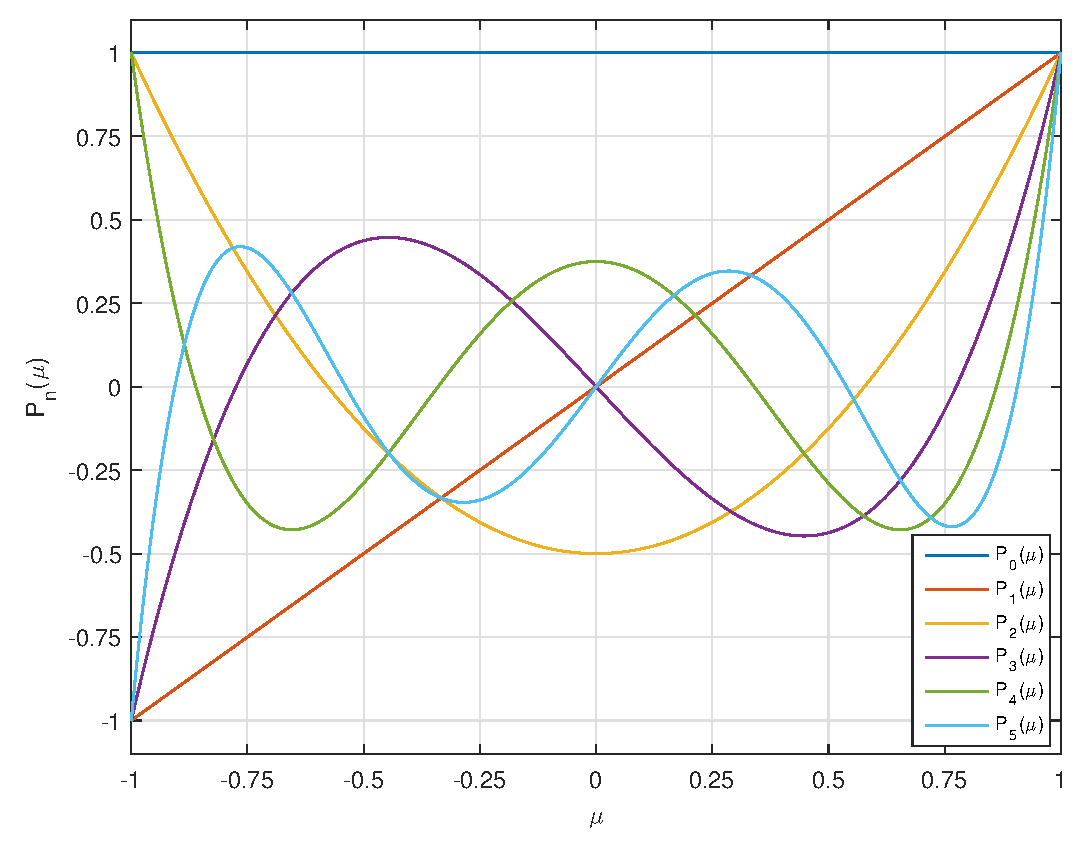
\includegraphics[width=\textwidth]{figures/appendices/LegPoly.eps}
\caption{Legendre polynomials of degrees 0 through 5.}
\label{fig::Legendre_Polynomials}
\end{figure}

An alternative definition for the spherical harmonics functions can be used that is more amenable to coding since there are no complex numbers involved. We can separate the spherical harmonics functions into their even ($Y_{n,k}^e  (\vec{\Omega}) $) and odd ($Y_{n,k}^o  (\vec{\Omega}) $) components. These definitions now have the form of 

\begin{equation}
\label{eq::App_SN_sharm_funcs}
\begin{aligned}
Y^e_{n,k} (\vec{\Omega}) &= \sqrt{C_{n,k}} P_n^k (\mu) \cos (k \theta), \qquad k=0,...,n  \\
Y^o_{n,k} (\vec{\Omega}) &= \sqrt{C_{n,k}} P_n^k (\mu) \sin (k \theta) , \qquad k=1,...,n
\end{aligned}
\end{equation}

\noindent where

\begin{equation}
\label{eq::App_SN_sharm_consts}
C_{n,k} = \frac{(n-k)!}{ (n+k) !}( 2-  \delta_{k,0}).
\end{equation}

\noindent The orthogonality condition applies to these functions:

\begin{equation}
\label{eq::App_SN_sharm_orth}
\begin{aligned}
\int\limits_{4 \pi} Y^e_{n,k} (\vec{\Omega}) Y^e_{m,l} (\vec{\Omega}) &= \frac{4 \pi}{2n+1} \delta_{n,m} \delta_{k,l} \\ 
\int\limits_{4 \pi} Y^o_{n,k} (\vec{\Omega}) Y^o_{m,l} (\vec{\Omega}) &= \frac{4 \pi}{2n+1} \delta_{n,m} \delta_{k,l} \\ 
\int\limits_{4 \pi} Y^e_{n,k} (\vec{\Omega}) Y^o_{m,l} (\vec{\Omega}) &= 0
\end{aligned} 
\end{equation}

\noindent The addition theorem is

\begin{equation}
\label{eq::App_SN_sharm_addition}
2 \pi P_n (\vec{\Omega}' \cdot \vec{\Omega}) = P_n (\mu_0) = \sum_{k=0}^{n} Y^e_{n,k} (\vec{\Omega}) Y^e_{n,k} (\vec{\Omega}') + \sum_{k=1}^{n} Y^o_{n,k} (\vec{\Omega}) Y^o_{n,k} (\vec{\Omega}') ,
\end{equation}

\noindent where

\begin{equation}
\label{eq::App_SN_mu_to_omegas}
\mu_0 \equiv \vec{\Omega}' \cdot \vec{\Omega} .
\end{equation}

\noindent We can then define the following angular flux moments as

\begin{equation}
\label{eq::App_SN_sharm_fluxmom}
\begin{aligned}
\Phi_{n,k,e} &=\int\limits_{4 \pi}\Psi (\vec{\Omega})  Y^e_{n,k} (\vec{\Omega})   \\ 
\Phi_{n,k,o} &=\int\limits_{4 \pi}\Psi (\vec{\Omega}) Y^o_{n,k} (\vec{\Omega}) 
\end{aligned} .
\end{equation}

\noindent With these flux moments, the angular flux can then be approximately expanded with the spherical harmonics functions:

\begin{equation}
\label{eq::App_SN_sharm_flux_exp}
\Psi(\vec{\Omega}) \approx \sum^{N_f}_{n=0} \frac{2n+1}{4 \pi} \left[ \sum_{k=0}^{n} \Phi_{n,k,e} Y^e_{n,k} (\vec{\Omega}) + \sum_{k=1}^{n} \Phi_{n,k,o} Y^o_{n,k} (\vec{\Omega})  \right] .
\end{equation}

\noindent where we have truncated the expansion to $N_f$. 

Now, we define the expansion of the scattering cross section by use of the Legendre polynomials. If we truncate at the $N_s$ term, the scattering cross section can be expanded as the following:

\begin{equation}
\label{eq::App_SN_scatt_exp}
\sigma_s (\mu_0) \approx \sum_{n=0}^{N_s} \frac{2n+1}{2} \sigma_{s,n} P_n (\mu_0) ,
\end{equation}

\noindent where 

\begin{equation}
\label{eq::App_SN_scatt_int}
\sigma_{s,n} \equiv \int\limits_{-1}^{1} d \mu_0 \, \sigma_s (\mu_0) P_n (\mu_0).
\end{equation}

If we define the term $N_p$ is the minimum integer value between $N_s$ and $N_f$, then we can then insert Eqs. (\ref{eq::App_SN_sharm_flux_exp}) and (\ref{eq::App_SN_scatt_int}) into Eq. (\ref{eq::App_SN_scatt_kernel}) to yield the following

\begin{equation}
\label{eq::App_SN_scatt_kernel_inserted}
\begin{aligned}
&\int\limits_{4 \pi} d \Omega' \, \sigma_s (\vec{\Omega}' \cdot \vec{\Omega}) \Psi (\vec{\Omega}')\\
= &\int\limits_{4 \pi} d \Omega'
\left\{ \begin{aligned}
&\left[\sum_{n=0}^{N_s} \frac{2n+1}{2} \sigma_{s,n} P_n (\vec{\Omega}' \cdot \vec{\Omega}) \right] \\
  &\left[\sum^{N_f}_{m=0} \frac{2m+1}{4 \pi} \left( \sum_{l=0}^{m} \Phi_{m,l,e} Y^e_{m,l} (\vec{\Omega}') + \sum_{l=1}^{m} \Phi_{m,l,o} Y^o_{m,l} (\vec{\Omega}')  \right) \right]
\end{aligned} \right\} \\
= &\int\limits_{4 \pi} d \Omega'
\left\{ \begin{aligned}
&\left[\sum_{n=0}^{N_s} \frac{2n+1}{2} \sigma_{s,n}\left[ \sum_{k=0}^{n} Y^e_{n,k} (\vec{\Omega}) Y^e_{n,k} (\vec{\Omega}') + \sum_{k=1}^{n} Y^o_{n,k} (\vec{\Omega}) Y^o_{n,k} (\vec{\Omega}') \right] \right]\\
  &\left[\sum^{N_f}_{m=0} \frac{2m+1}{4 \pi} \left( \sum_{l=0}^{m} \Phi_{m,l,e} Y^e_{m,l} (\vec{\Omega}') + \sum_{l=1}^{m} \Phi_{m,l,o} Y^o_{m,l} (\vec{\Omega}')  \right) \right]
\end{aligned} \right\} \\
=&\sum_{n=0}^{N_p} \frac{2n+1}{4 \pi}\sigma_{s,n} \left[  \sum_{k=0}^{n} \Phi_{n,k,e} Y^e_{n,k} (\vec{\Omega}) + \sum_{k=1}^{n} \Phi_{n,k,o} Y^o_{n,k} (\vec{\Omega})  \right]
\end{aligned}
\end{equation}

\noindent To ease notation, let us define the following:

\begin{equation}
\label{eq::App_SN_sharm_flux_ease}
\begin{aligned}
Y_{n,k} (\vec{\Omega}) &\equiv Y_{n,k}^e (\vec{\Omega}), & k=0,...,n\\
Y_{n,-k} (\vec{\Omega}) &\equiv Y_{n,k}^o (\vec{\Omega}), & k=1,...,n\\
\Phi_{n,k} &\equiv \Phi_{n,k,e}, & k=0,...,n\\ 
\Phi_{n,-k} &\equiv\Phi_{n,k,o}, & k=1,...,n
\end{aligned} 
\end{equation}

\noindent With this simplification, we can write the final form for the scattering kernel:

\begin{equation}
\label{eq::App_SN_scatt_kernel_FINAL}
\int\limits_{4 \pi} d \Omega' \, \sigma_s (\vec{\Omega}' \cdot \vec{\Omega}) \Psi (\vec{\Omega}')  = \sum_{n=0}^{N_p} \frac{2n+1}{4 \pi}\sigma_{s,n} \sum_{k=-n}^{n} \Phi_{n,k} Y_{n,k} (\vec{\Omega})
\end{equation}


% List of Spherical Harmonics Plots
\iffalse
\pagebreak

\begin{figure}
\label{fig::Sn_Y0}
\centering
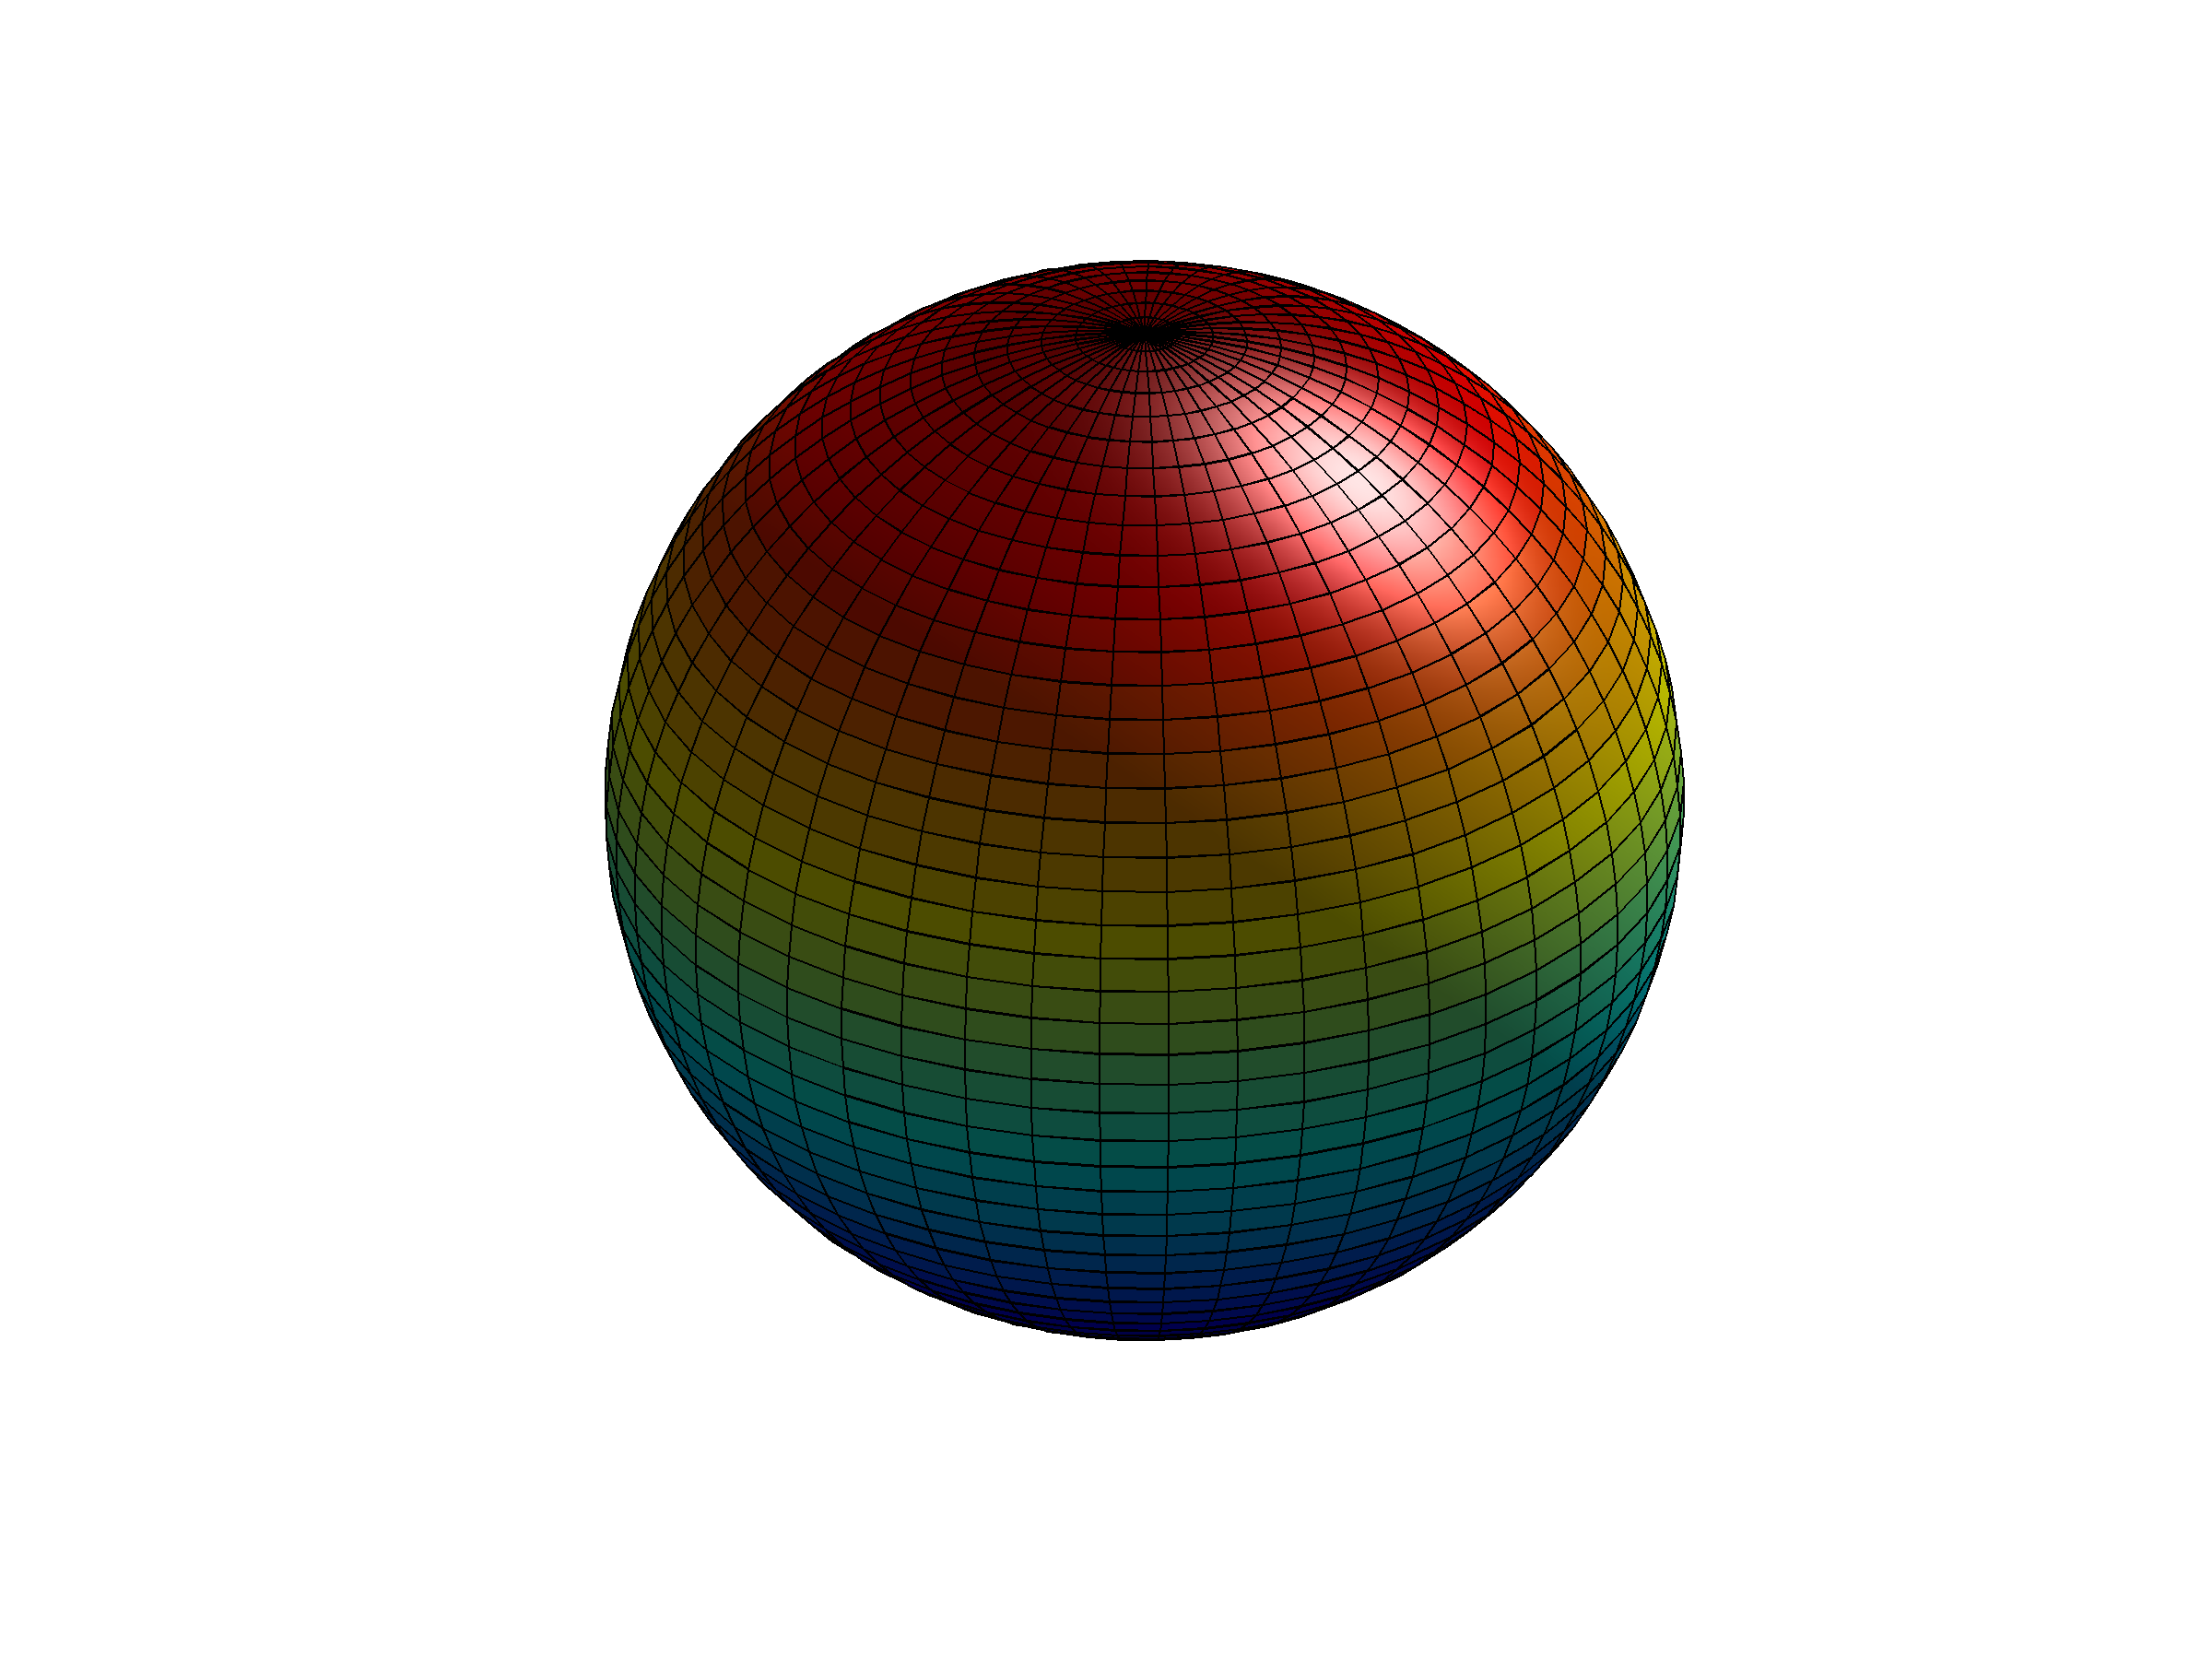
\includegraphics[width=0.45\textwidth]{figures/appendices/Y_0_0.png}
\caption{Spherical harmonic function of degree 0: $Y_{0}^{0}$.}
\end{figure}

\begin{figure}
\label{fig::Sn_Y1}
\centering
	\begin{subfigure}[b]{0.45\textwidth}
		\centering
		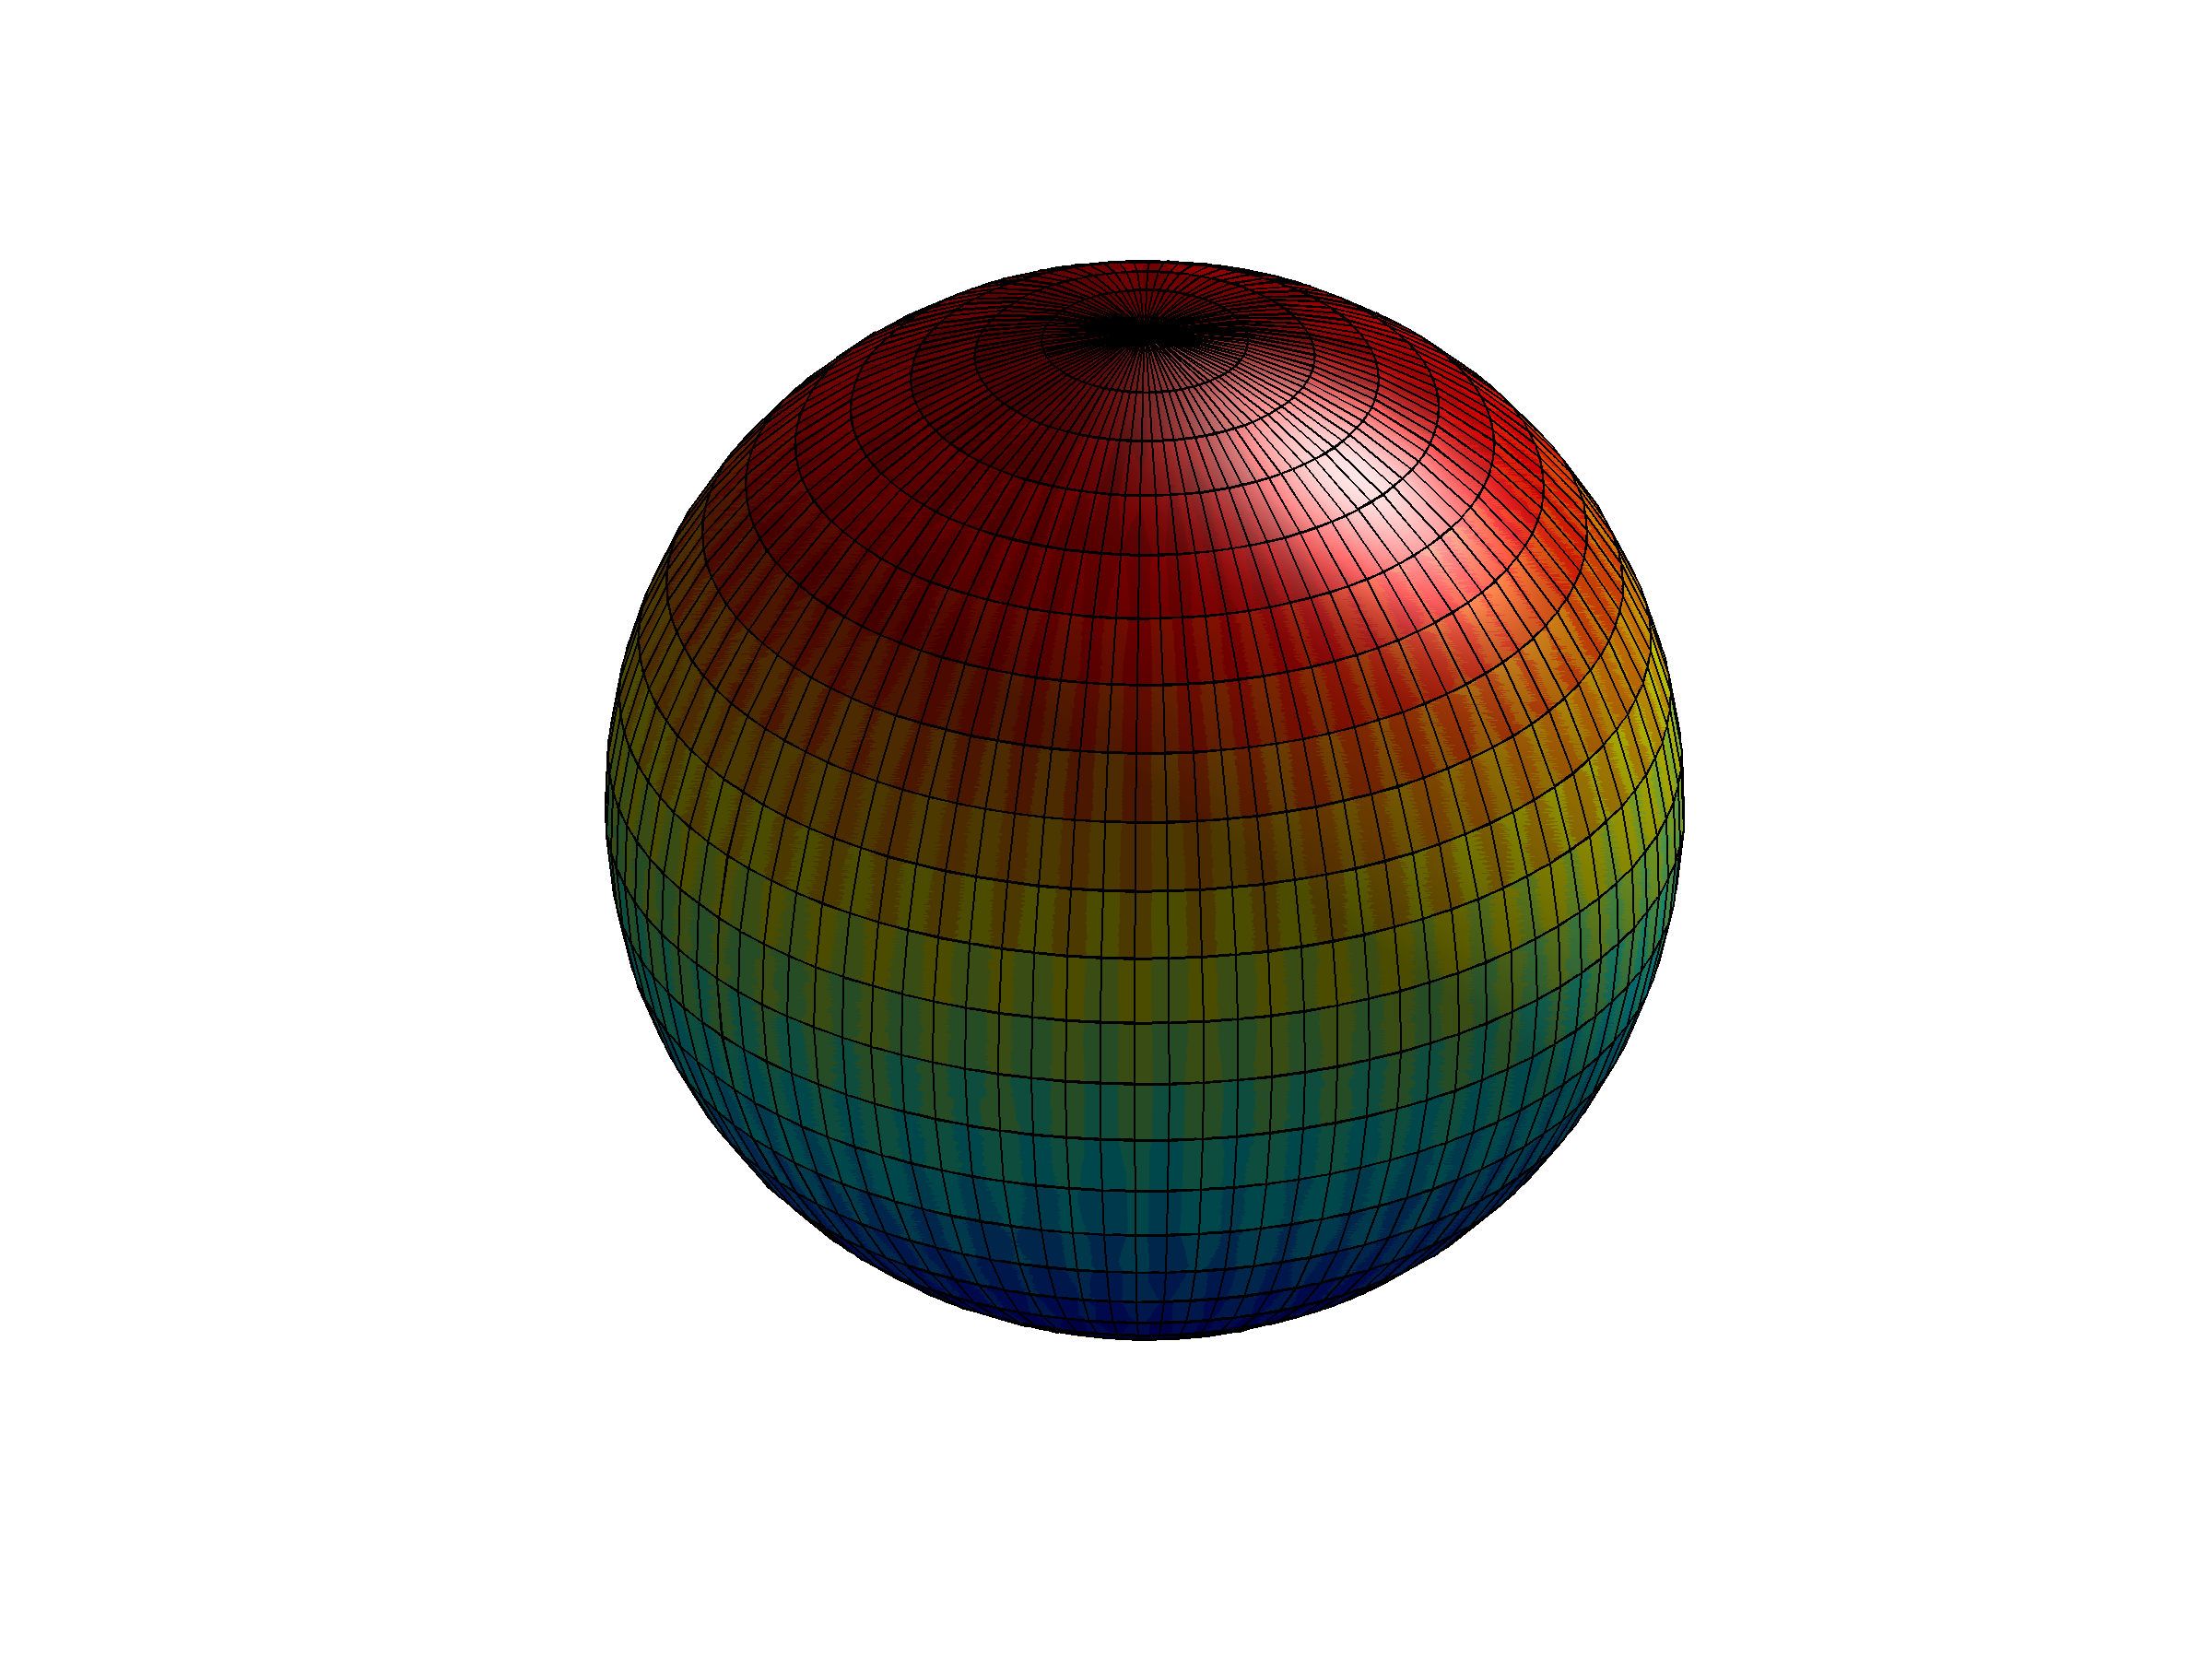
\includegraphics[width=\textwidth]{figures/appendices/Y_1_0.png}
		\caption{}
	\end{subfigure}
	\vfill
	\begin{subfigure}[b]{0.40\textwidth}
		\centering
		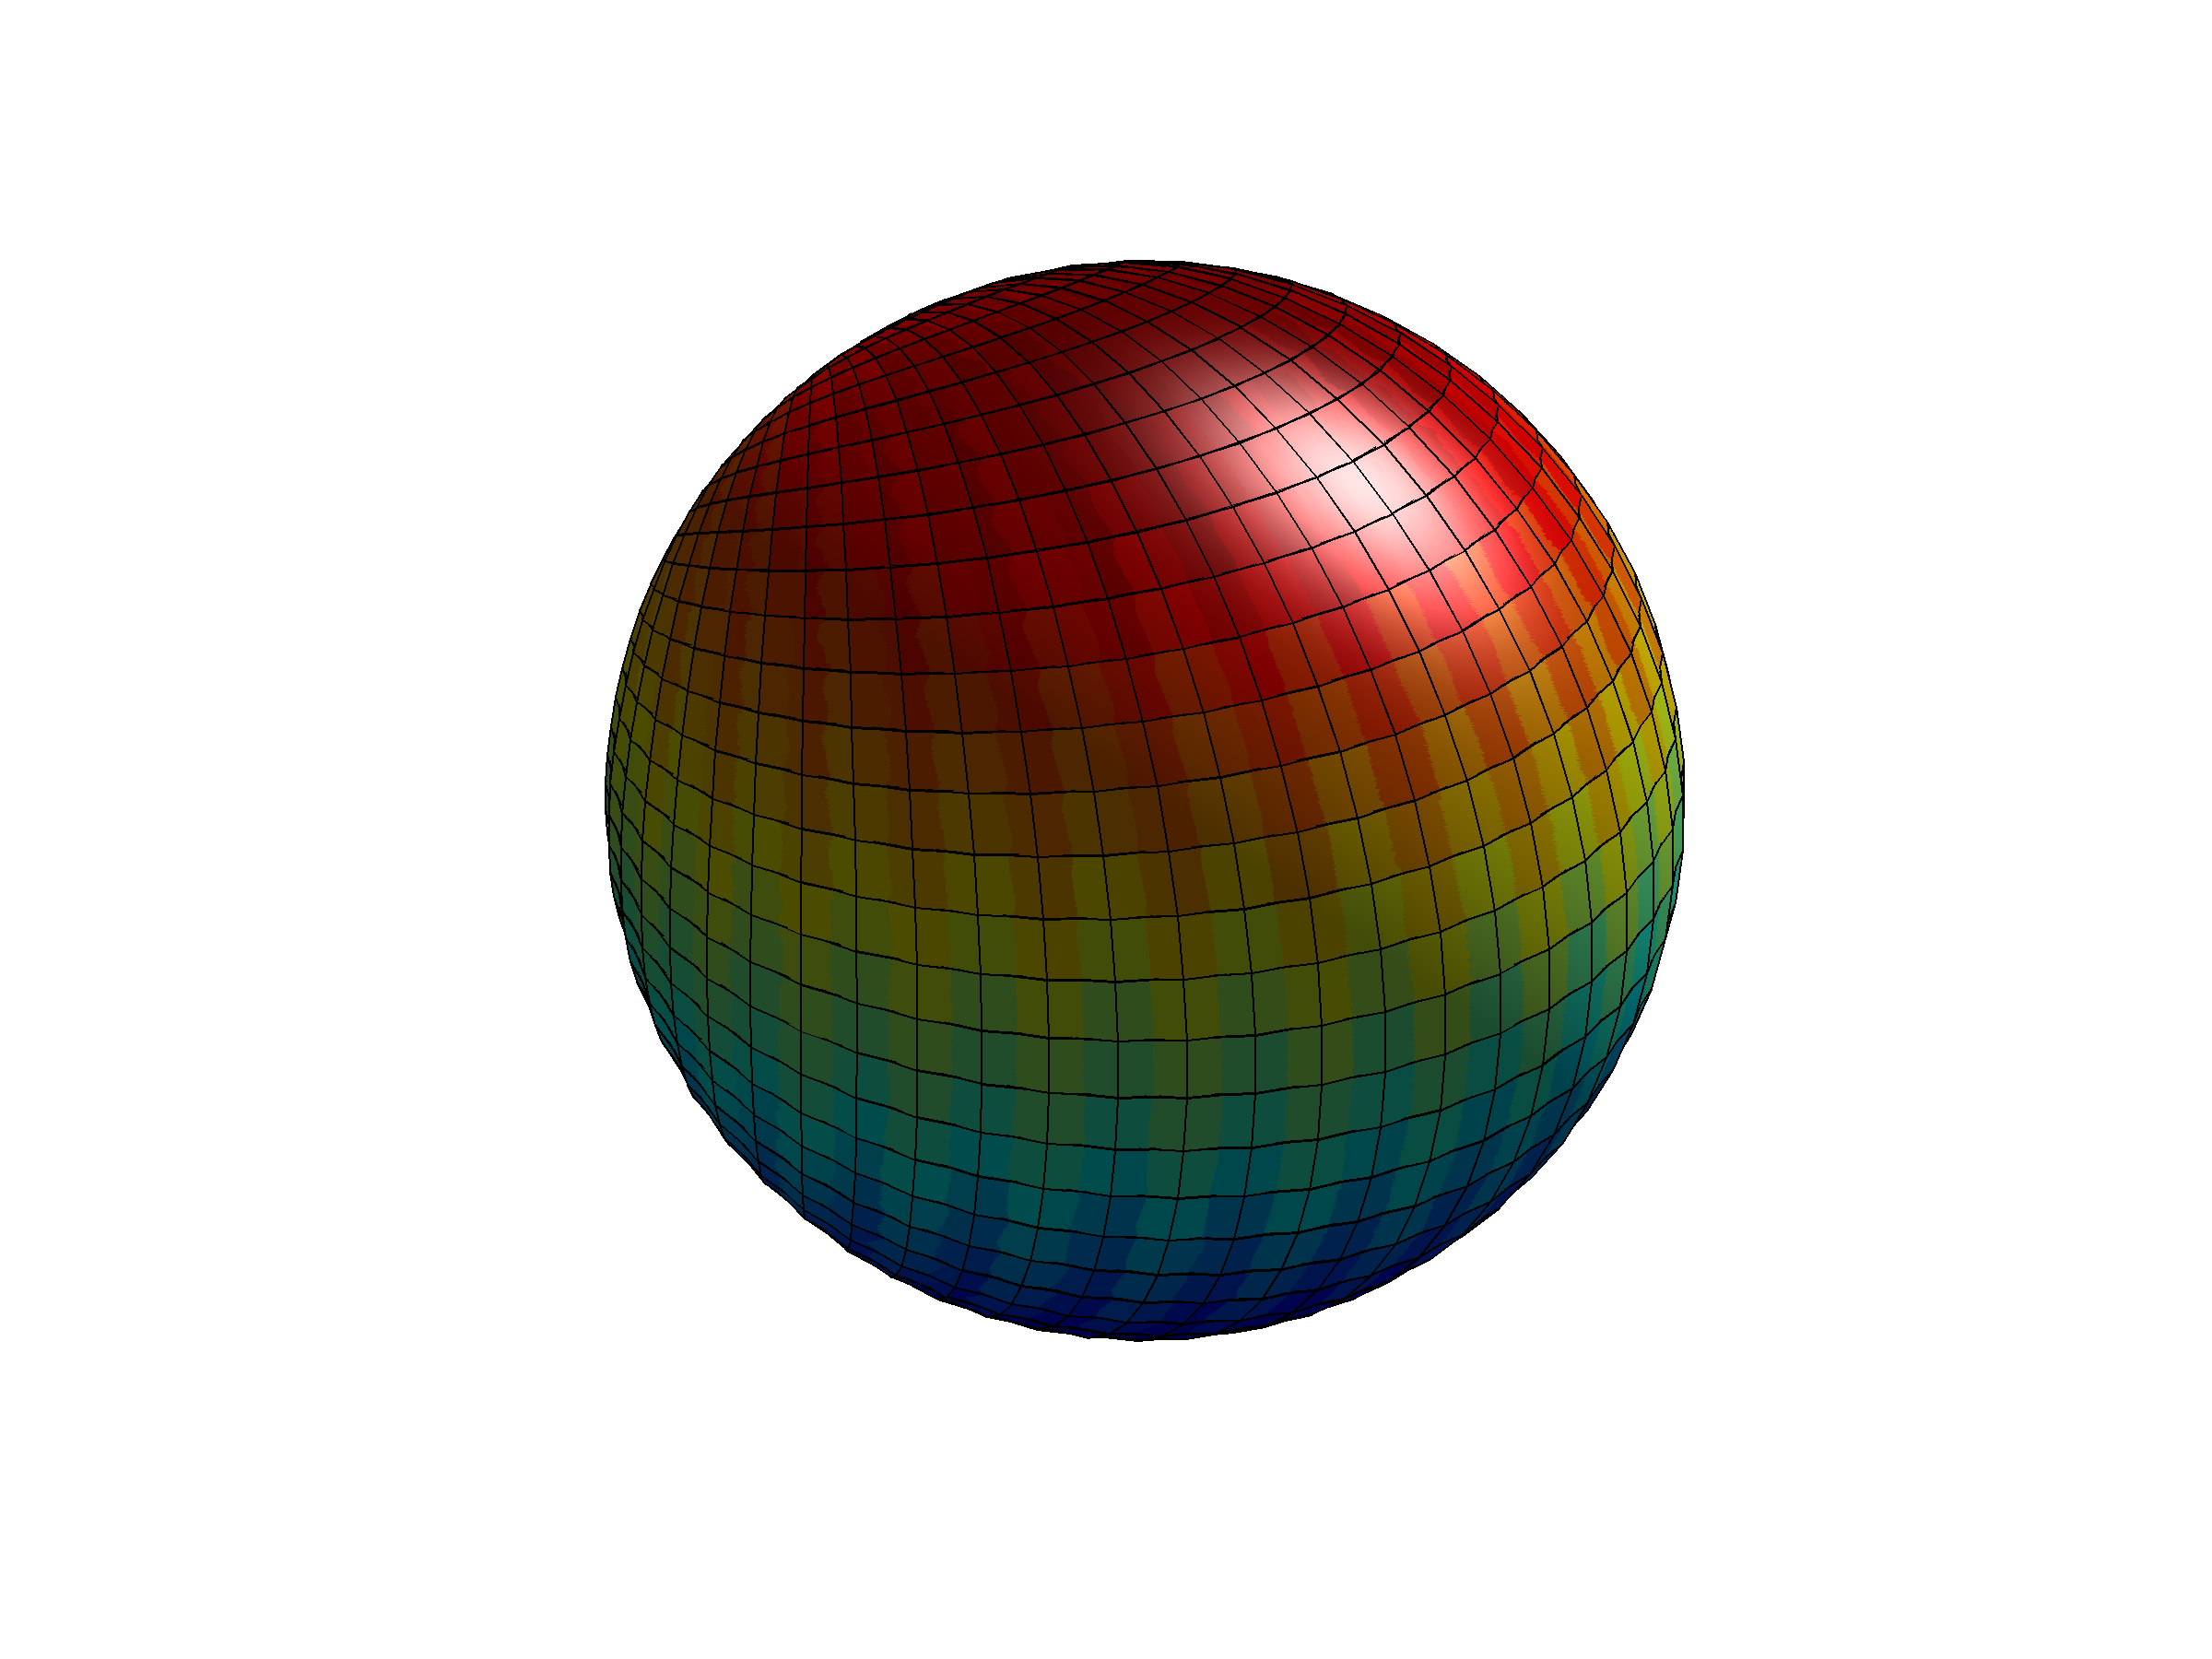
\includegraphics[width=\textwidth]{figures/appendices/Y_1_-1.png}
		\caption{}
	\end{subfigure}
	\hfill
	\begin{subfigure}[b]{0.40\textwidth}
		\centering
		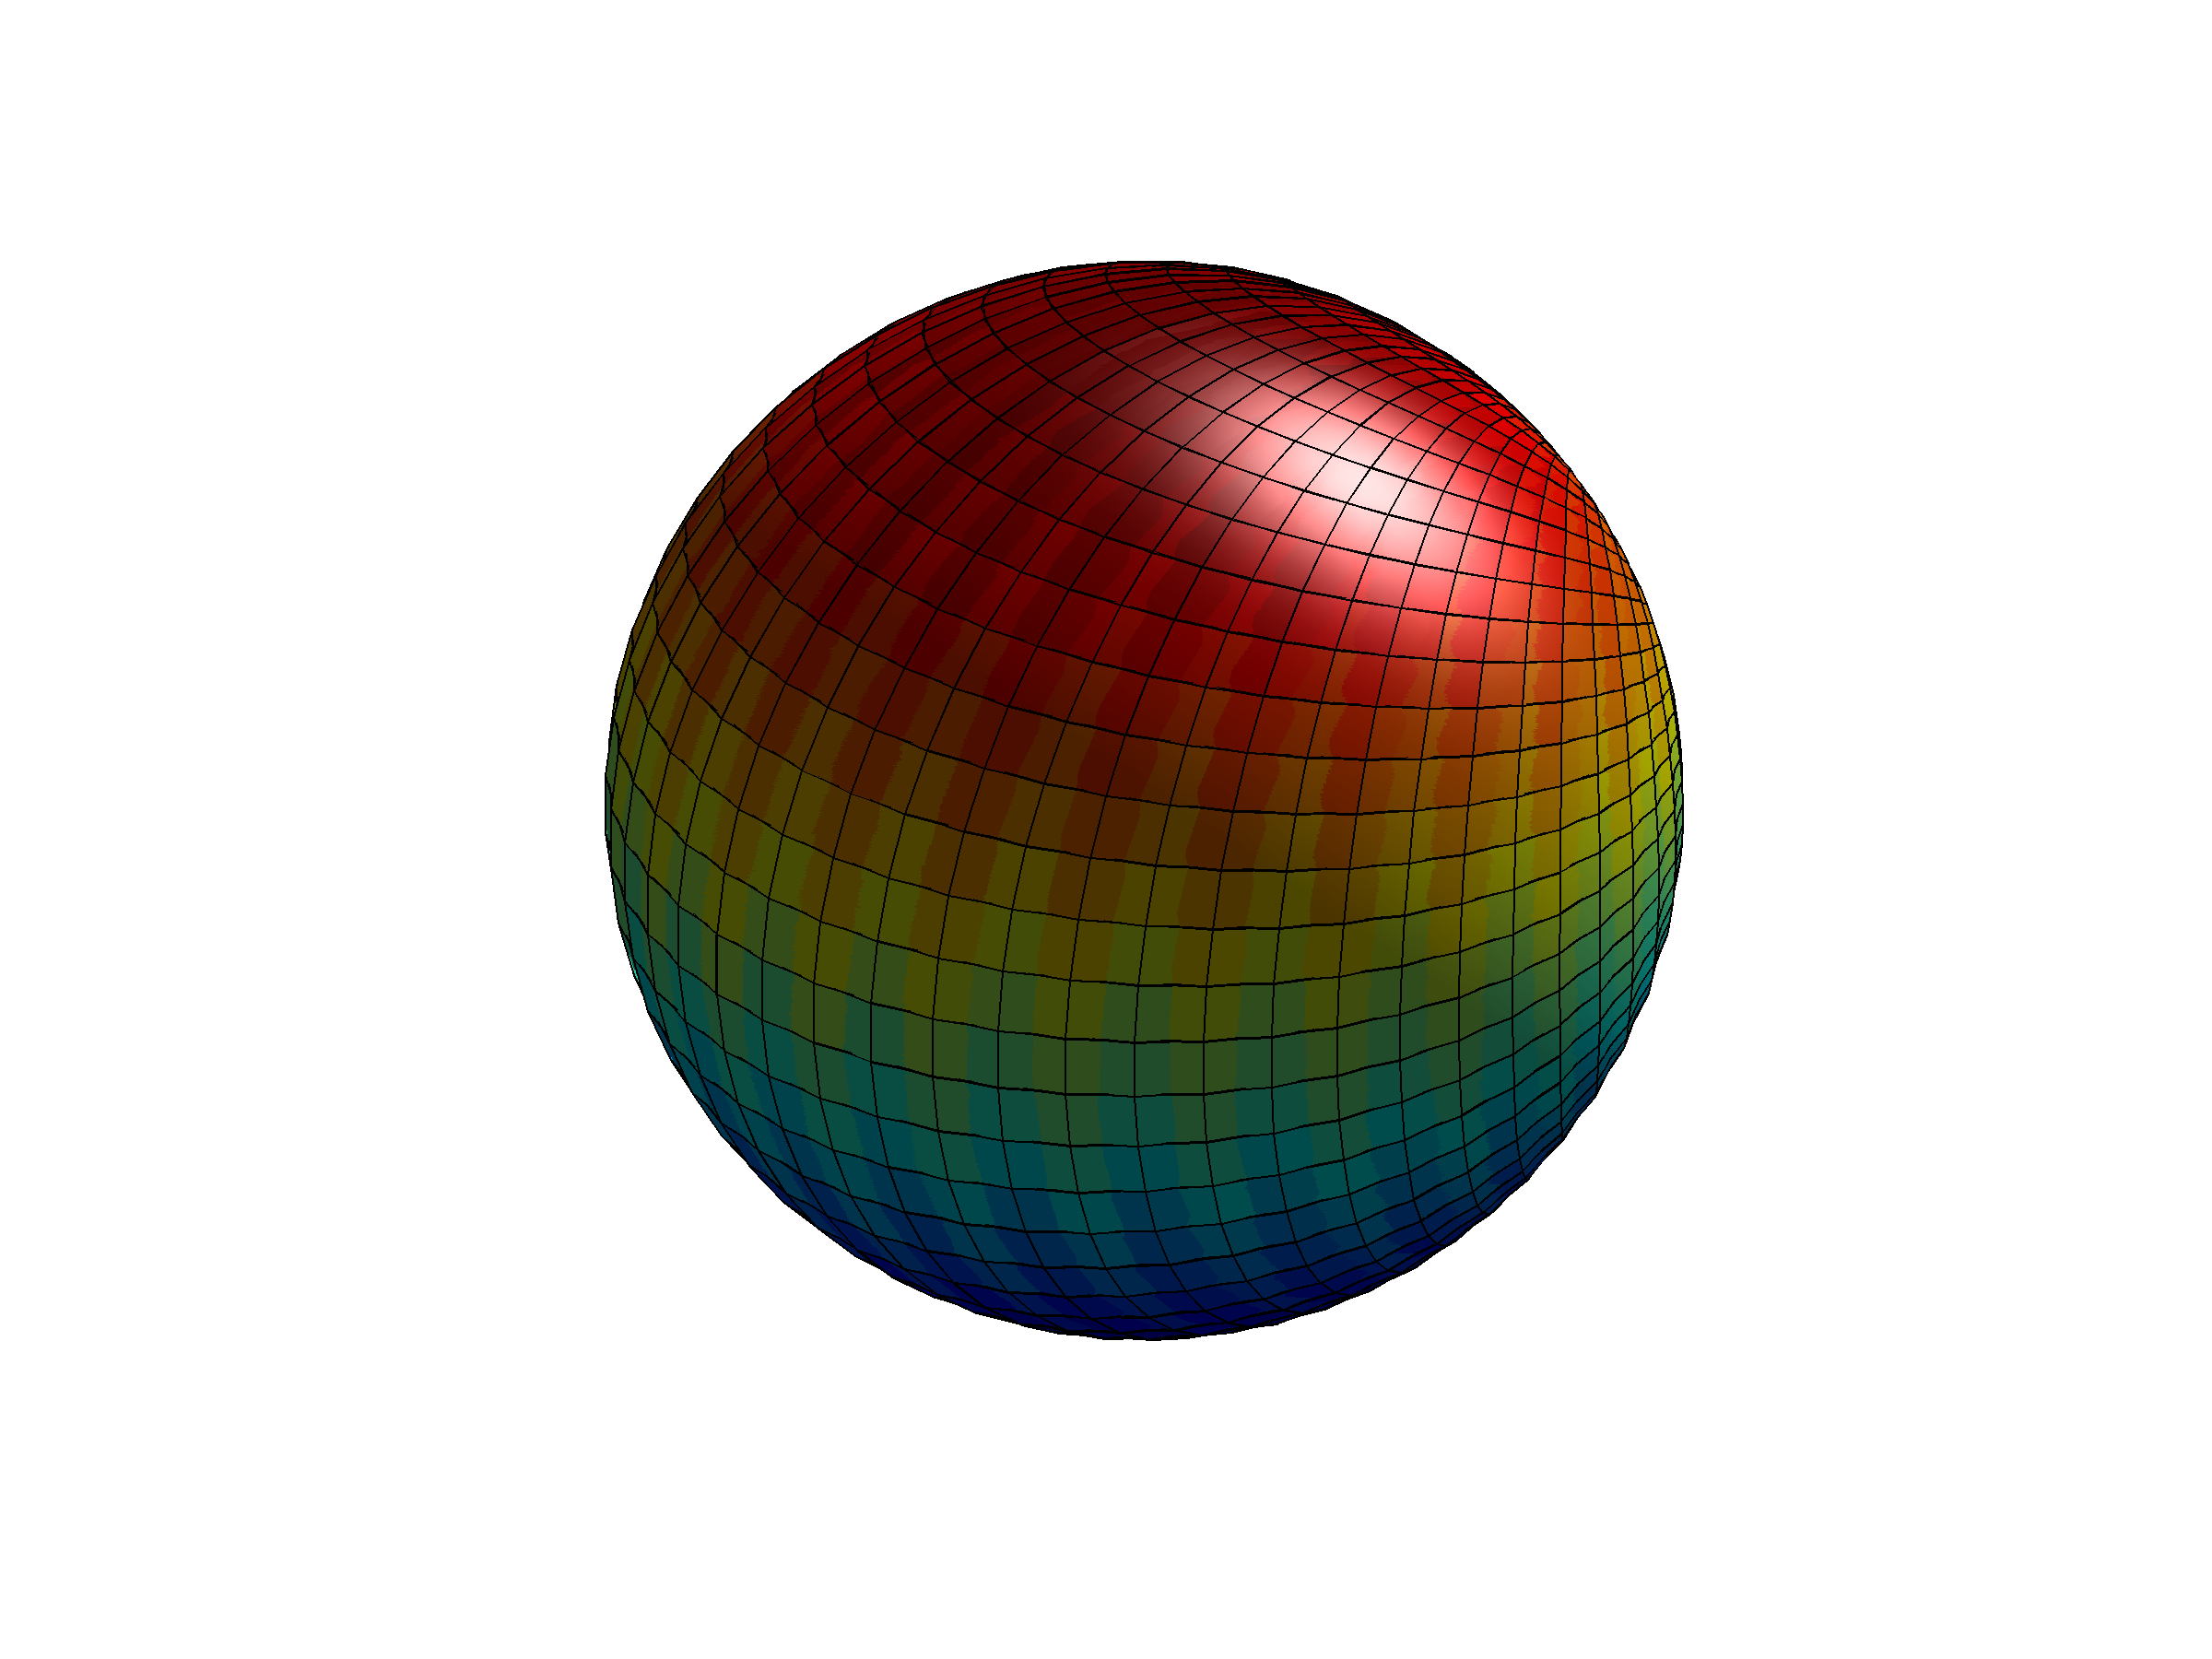
\includegraphics[width=\textwidth]{figures/appendices/Y_1_1.png}
		\caption{}
	\end{subfigure}
\caption{Spherical harmonic functions of degree 1: (a) $Y_{1}^{0}$, (b) $Y_{1}^{-1}$, and (c) $Y_{1}^{1}$.}
\end{figure}

\begin{figure}
\label{fig::Sn_Y2}
\centering
	\begin{subfigure}[b]{0.45\textwidth}
		\centering
		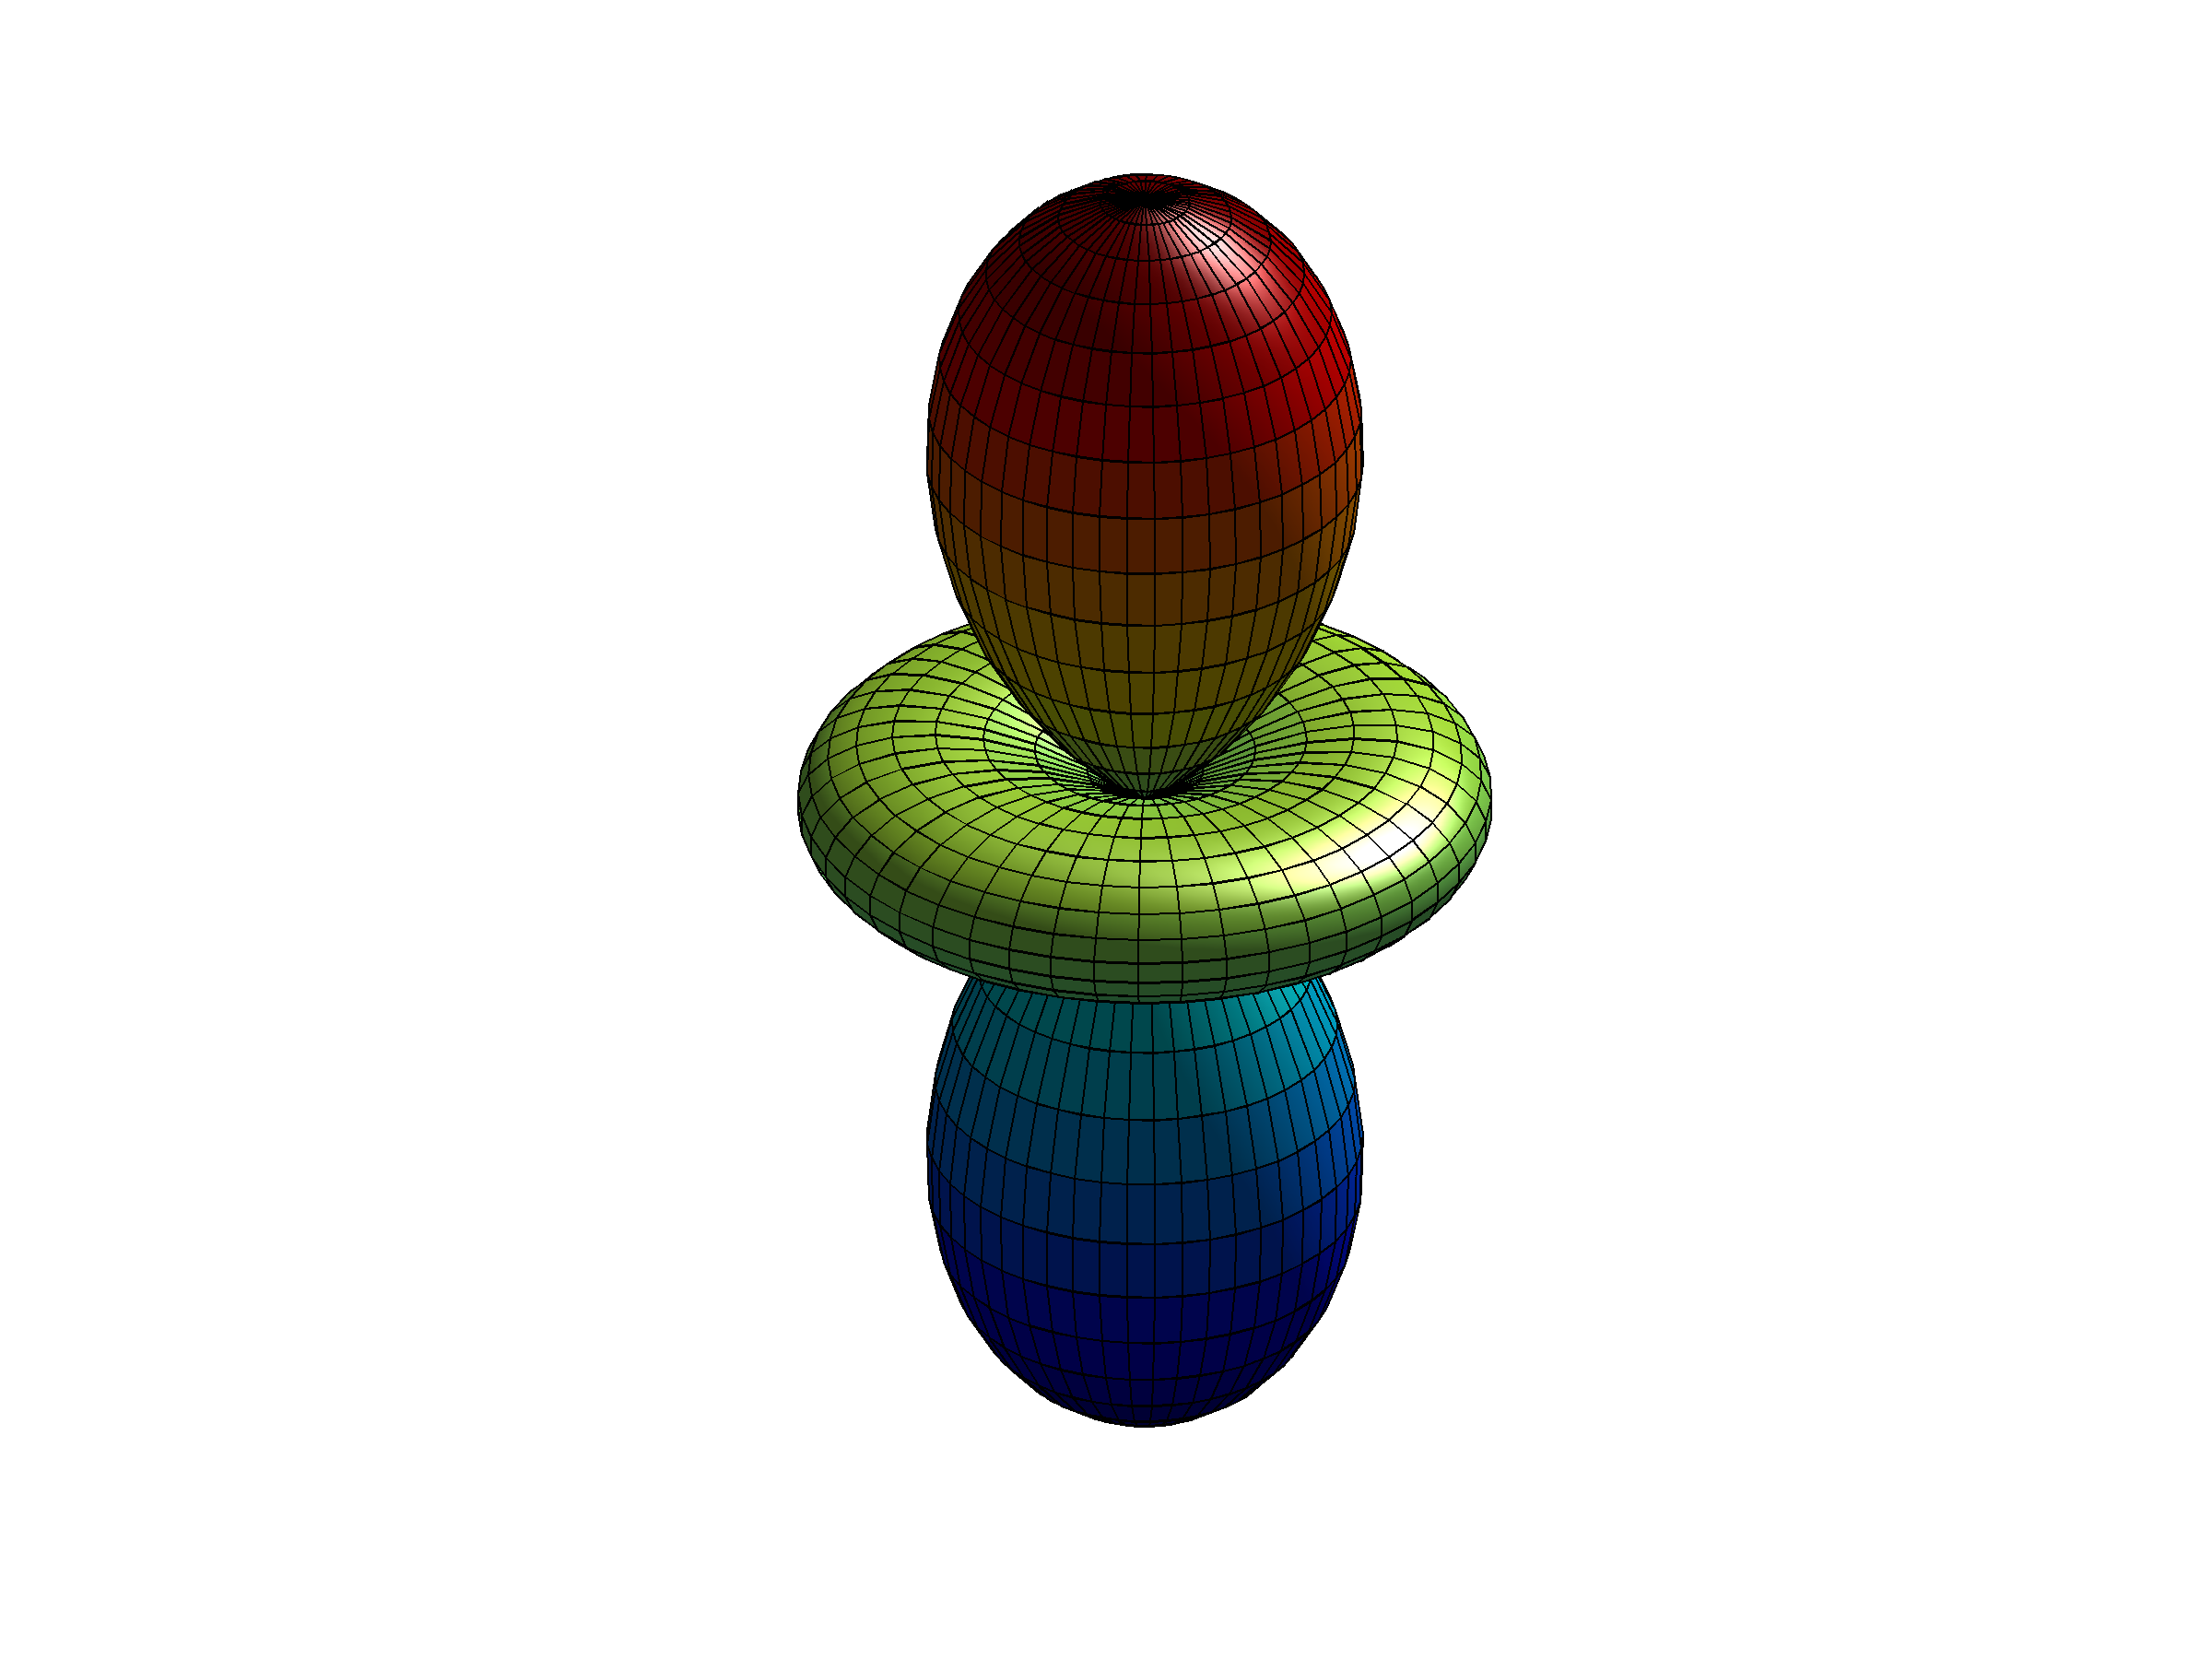
\includegraphics[width=\textwidth]{figures/appendices/Y_2_0.png}
		\caption{}
	\end{subfigure}
	\vfill
	\begin{subfigure}[b]{0.40\textwidth}
		\centering
		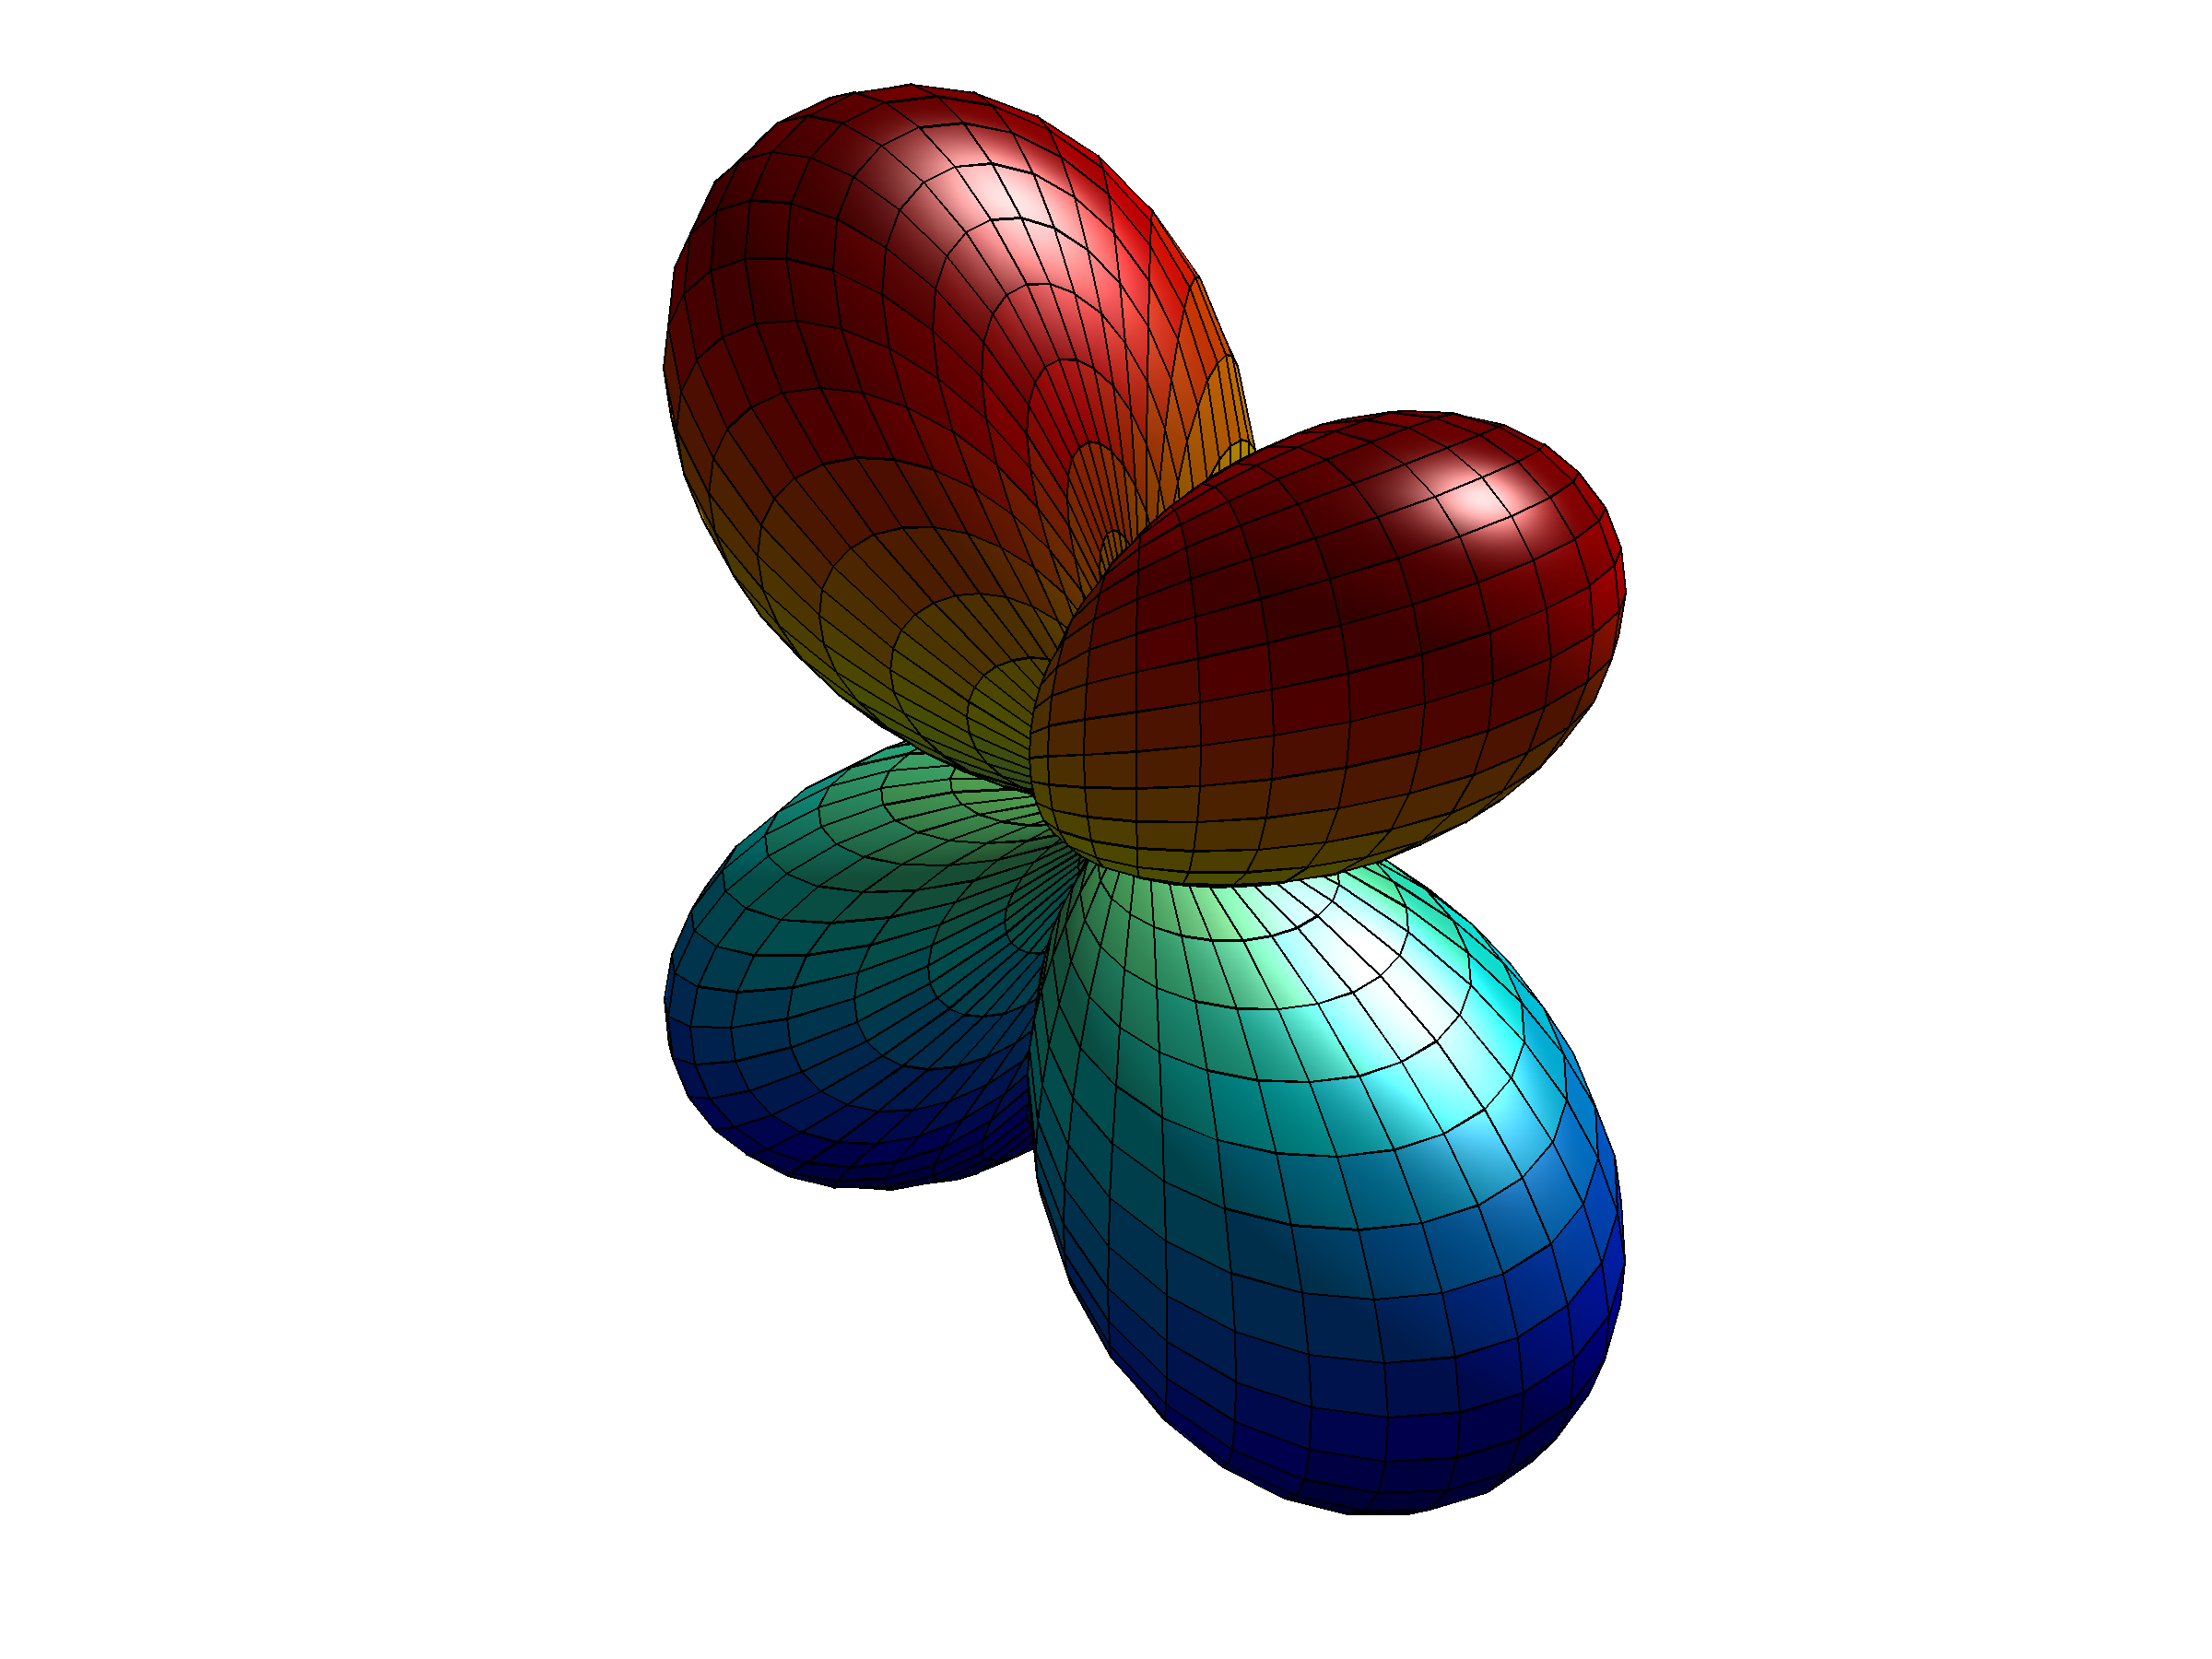
\includegraphics[width=\textwidth]{figures/appendices/Y_2_-1.png}
		\caption{}
	\end{subfigure}
	\hfill
	\begin{subfigure}[b]{0.40\textwidth}
		\centering
		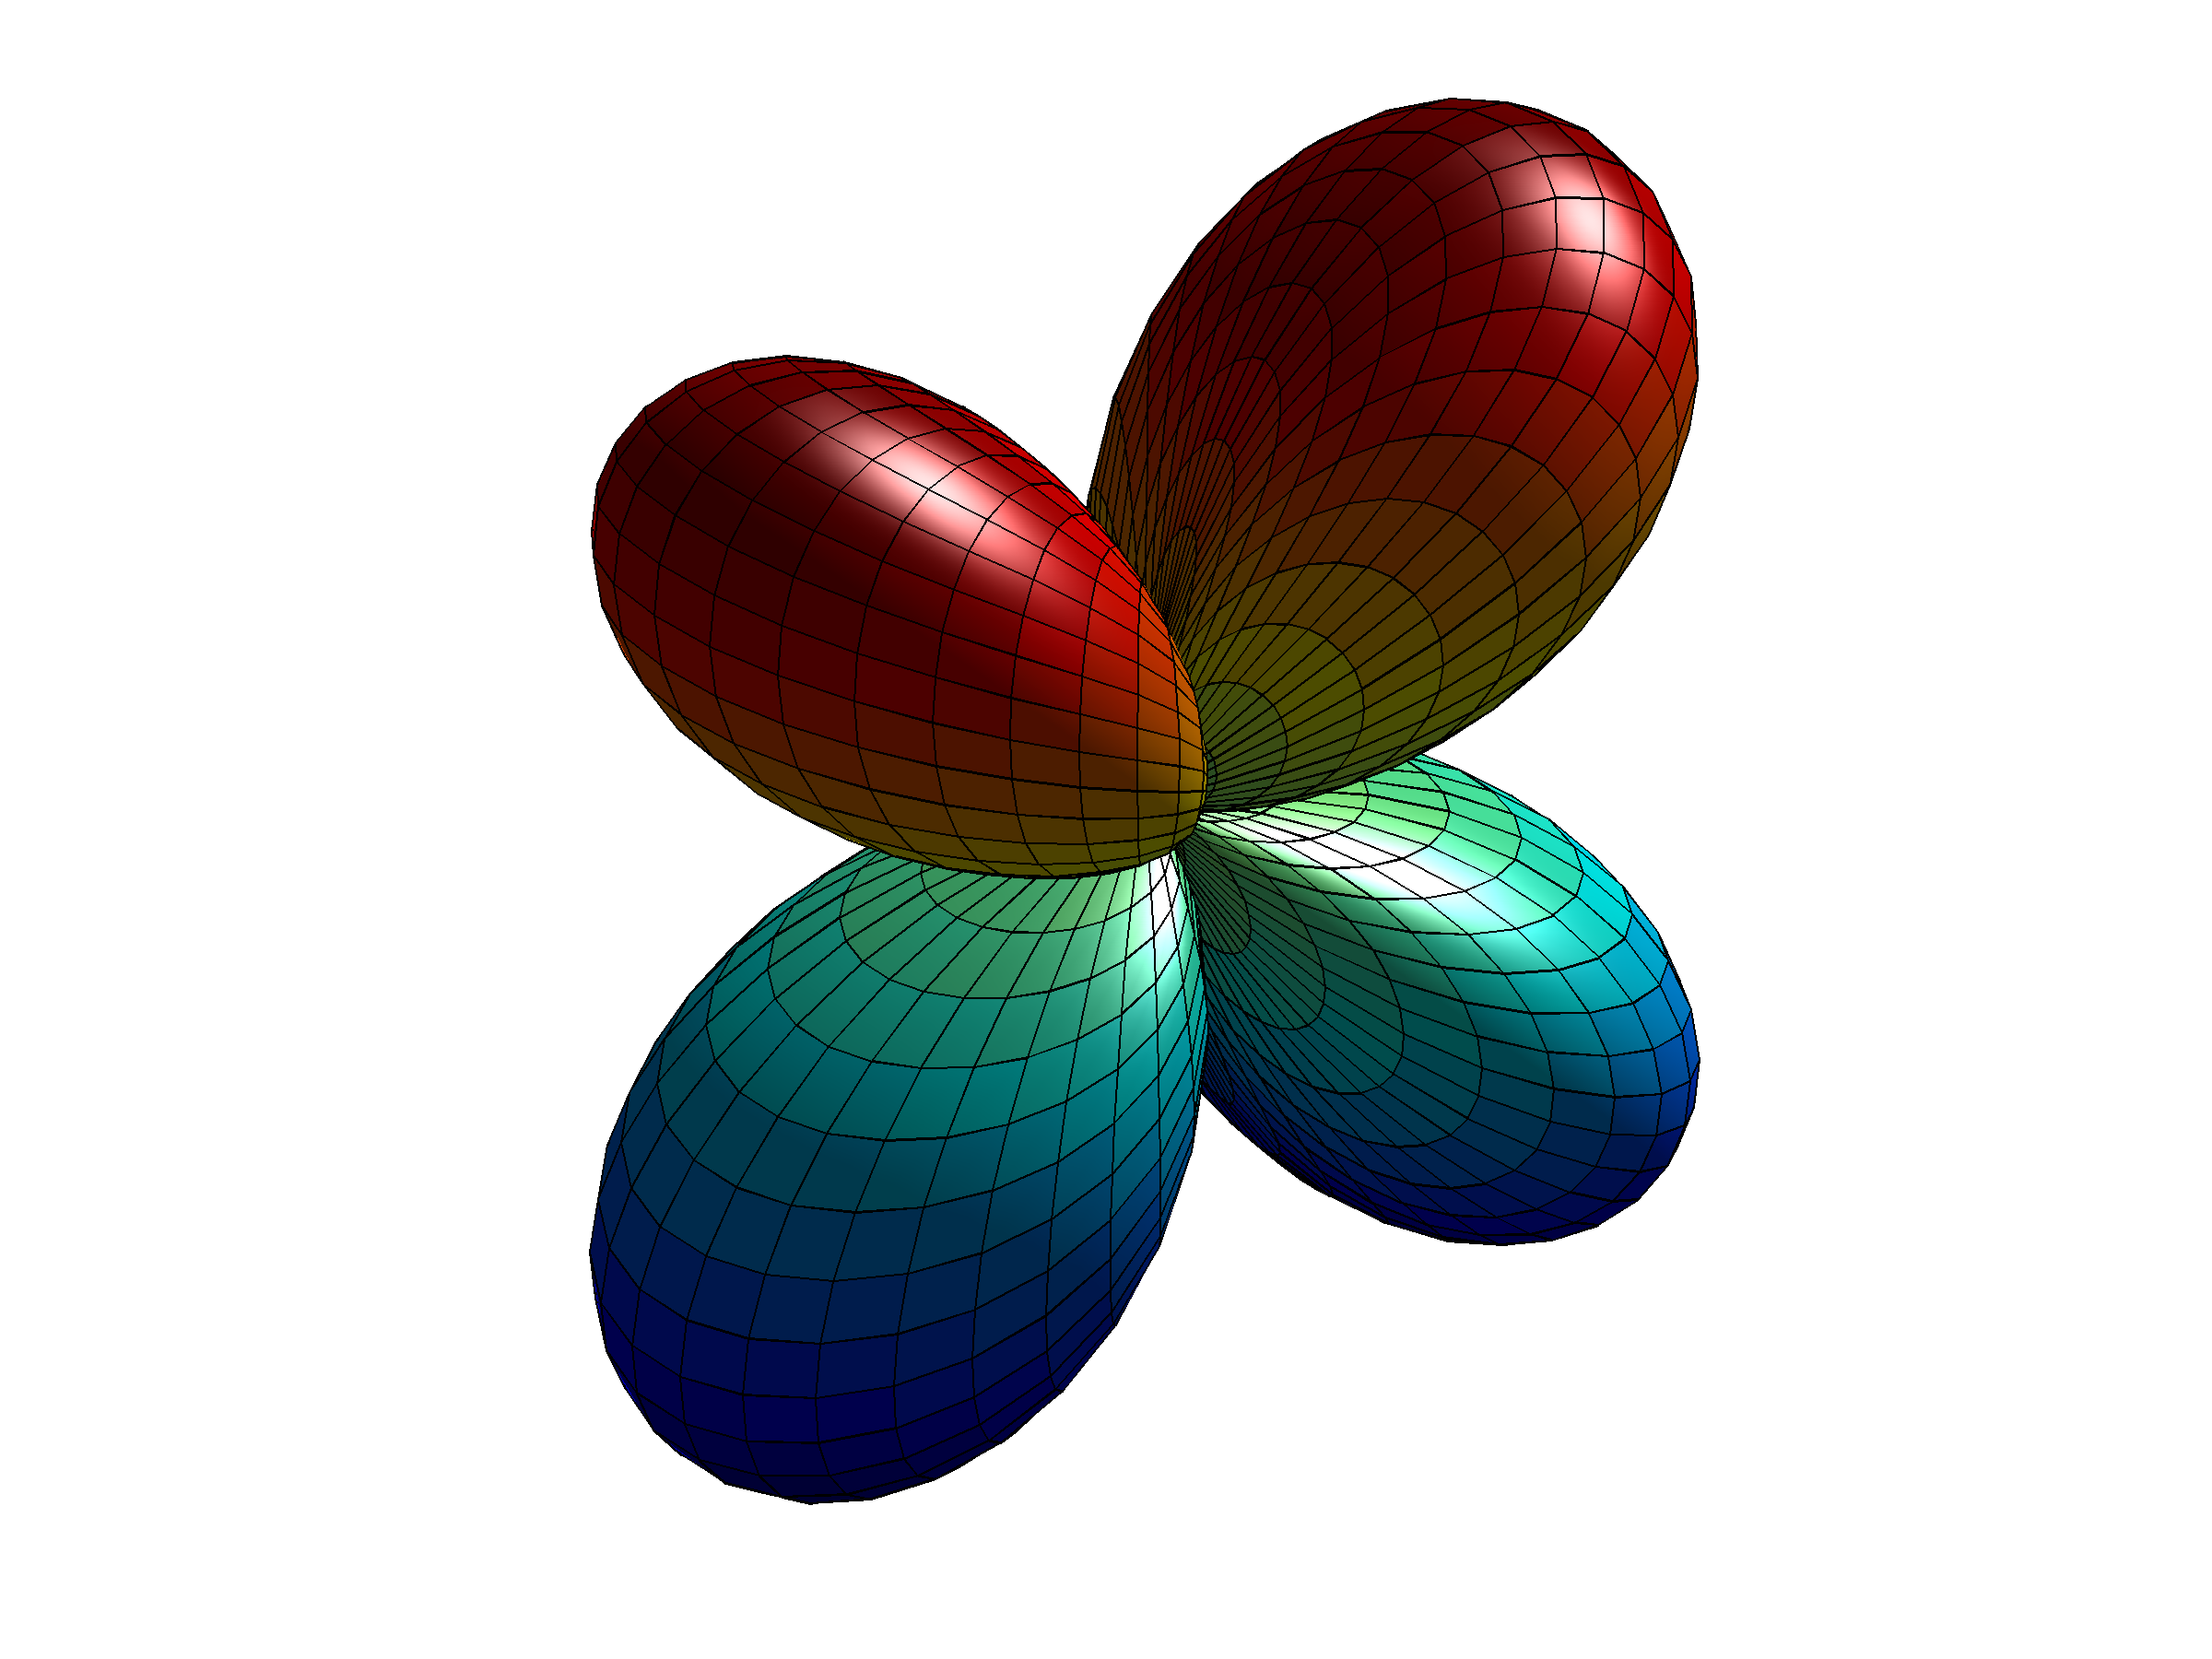
\includegraphics[width=\textwidth]{figures/appendices/Y_2_1.png}
		\caption{}
	\end{subfigure}
	\vfill
	\begin{subfigure}[b]{0.40\textwidth}
		\centering
		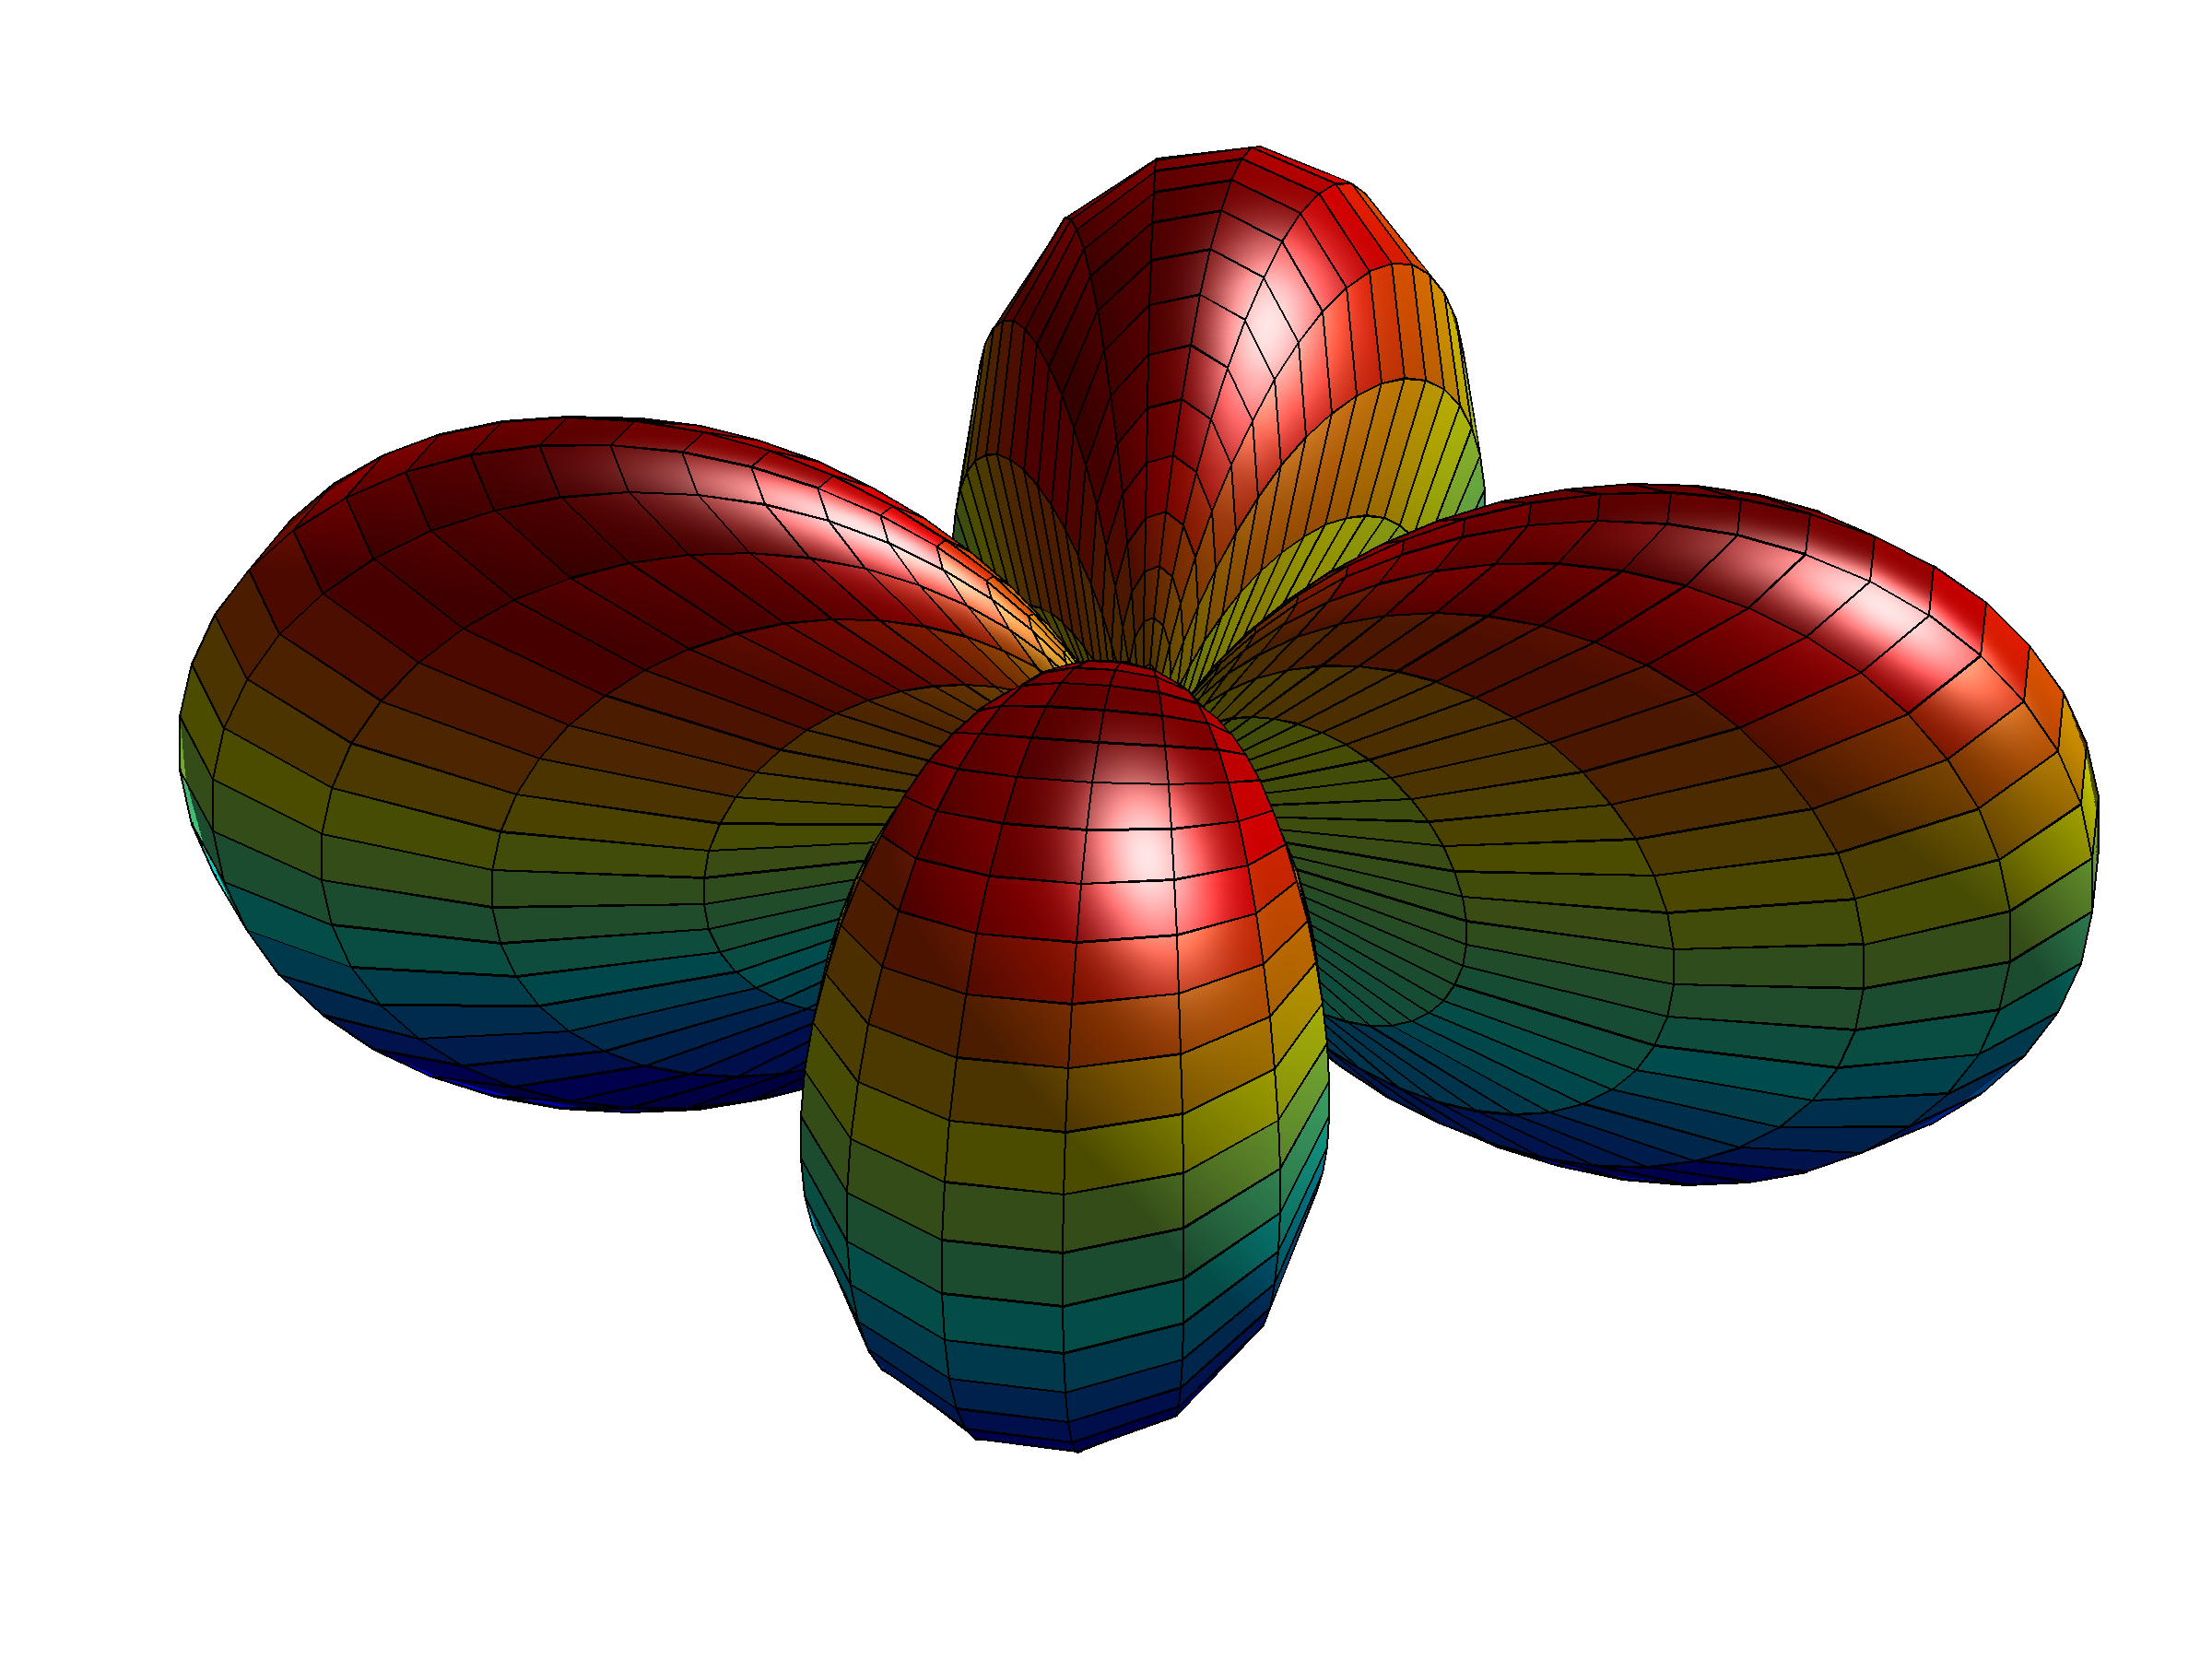
\includegraphics[width=\textwidth]{figures/appendices/Y_2_-2.png}
		\caption{}
	\end{subfigure}
	\hfill
	\begin{subfigure}[b]{0.40\textwidth}
		\centering
		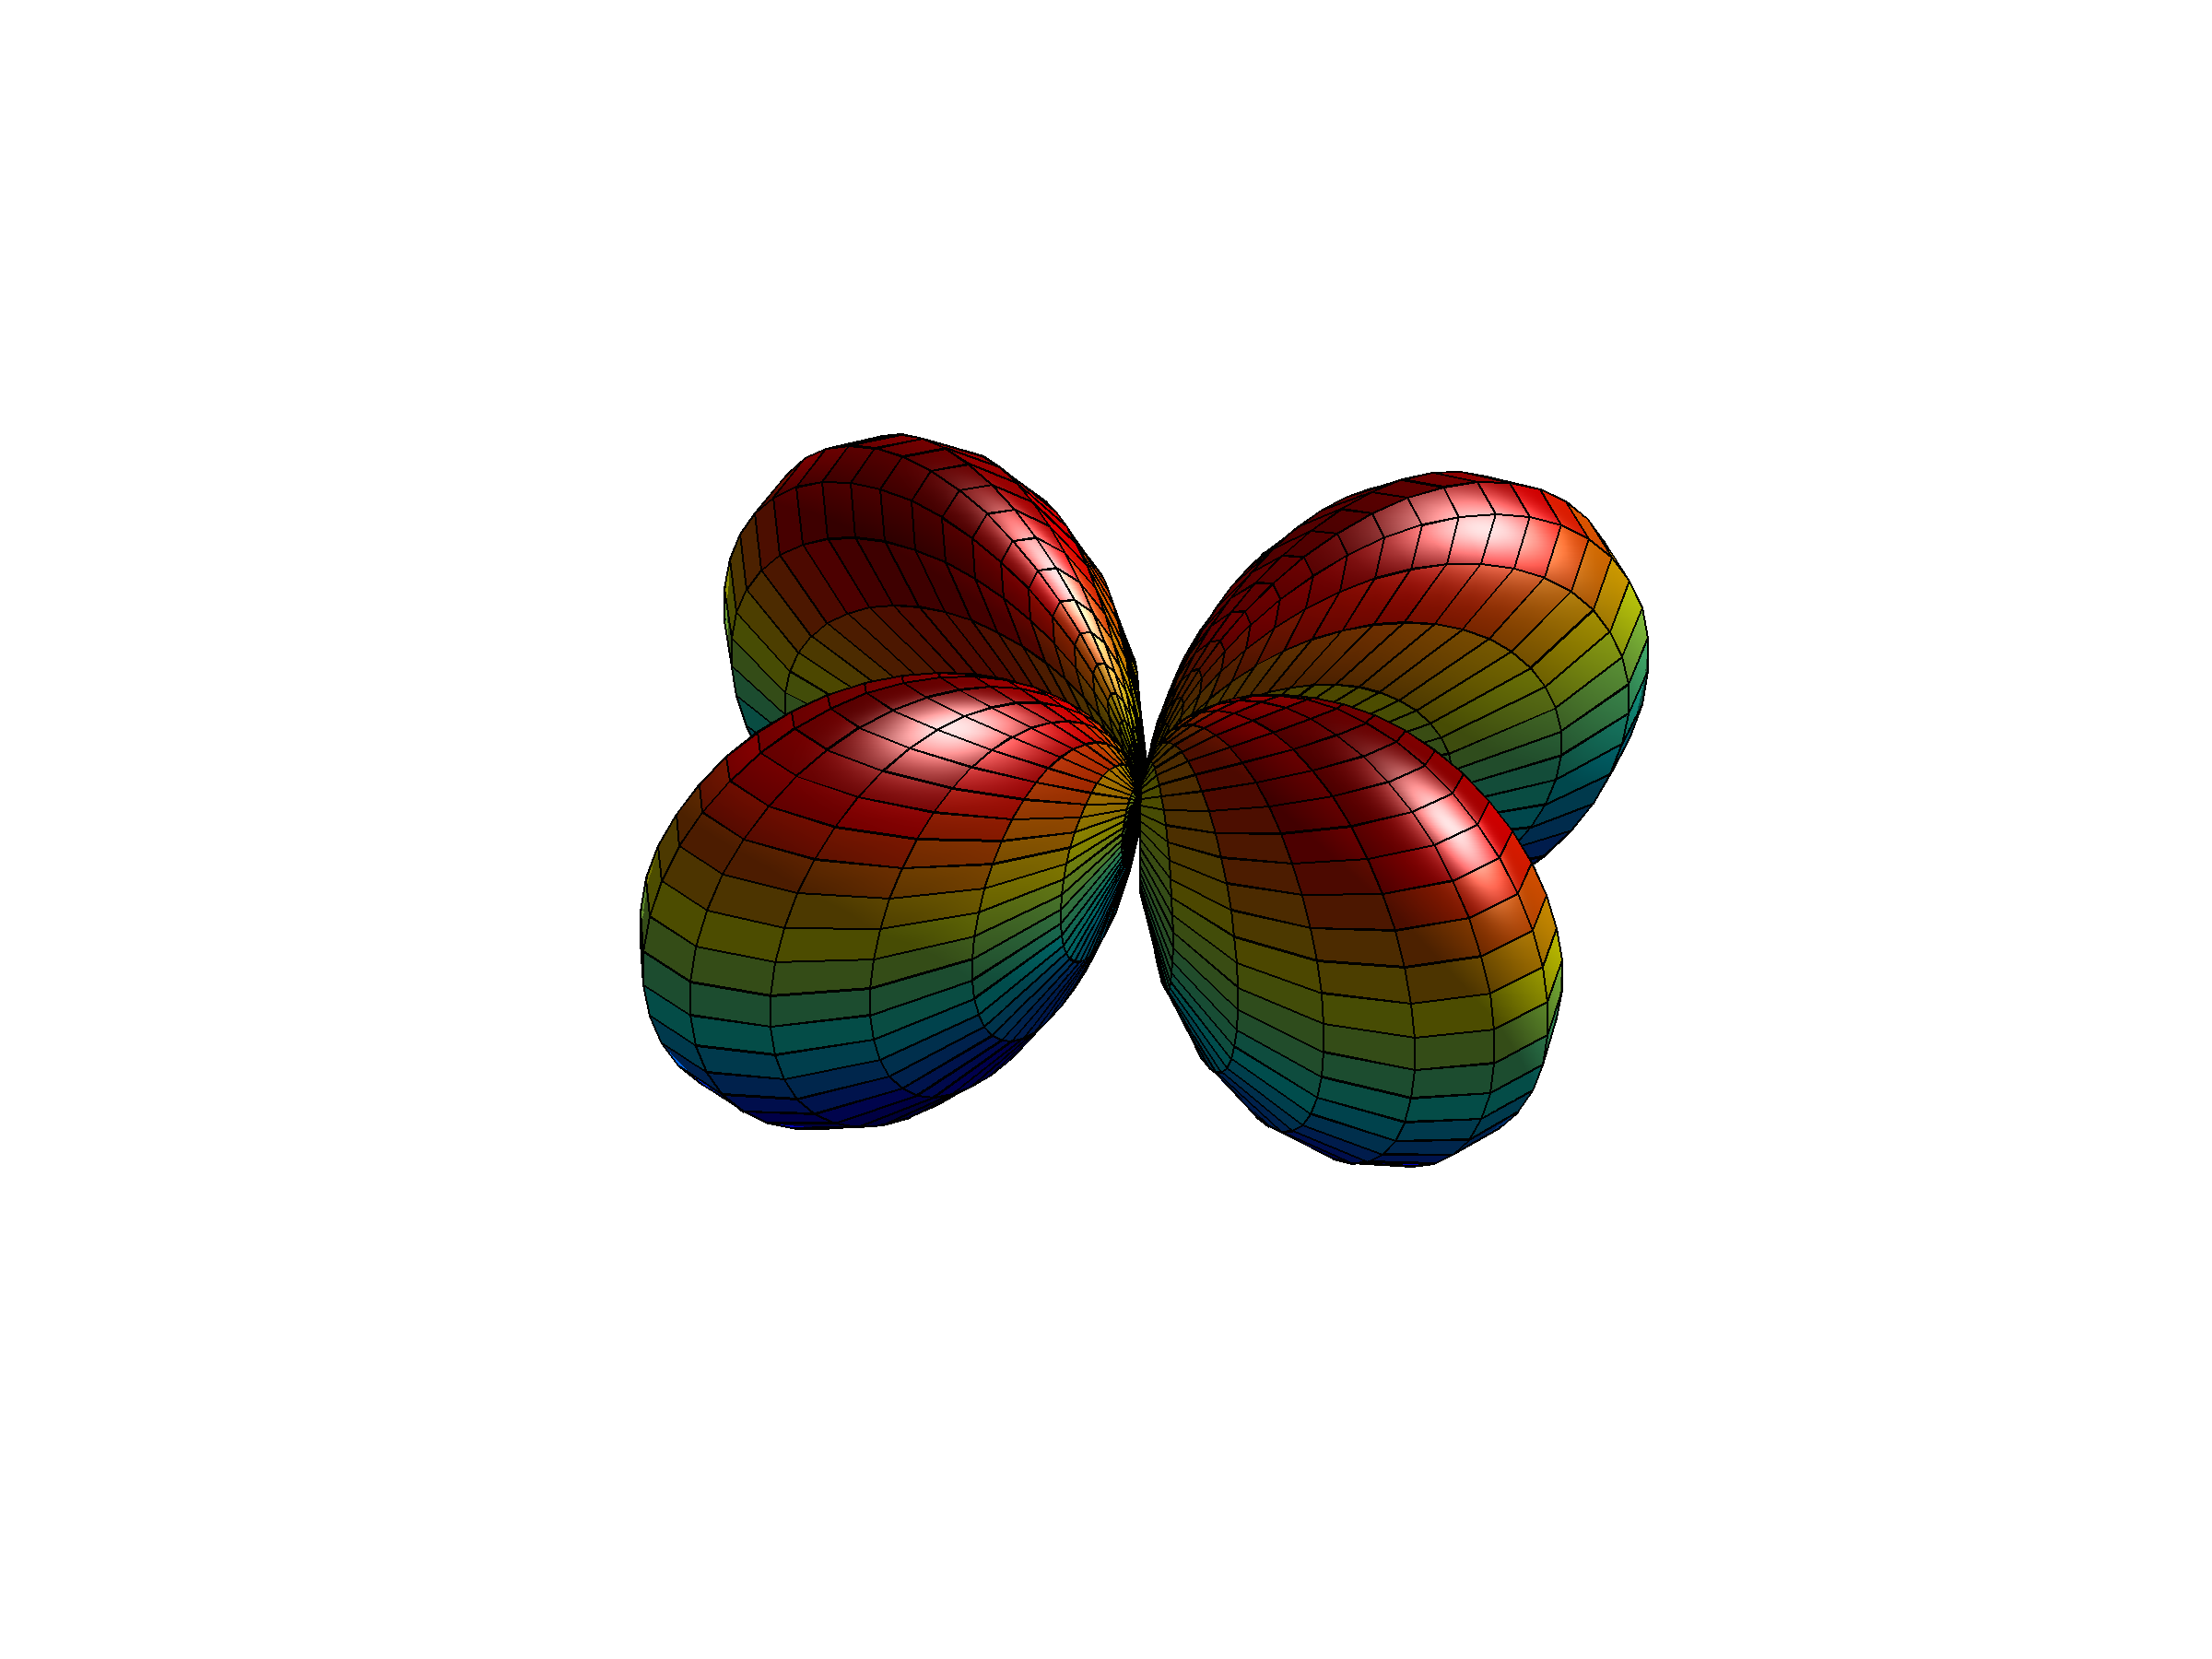
\includegraphics[width=\textwidth]{figures/appendices/Y_2_2.png}
		\caption{}
	\end{subfigure}
\caption{Spherical harmonic functions of degree 2: (a) $Y_{2}^{0}$, (b) $Y_{2}^{-1}$, (c) $Y_{2}^{1}$, (d) $Y_{2}^{-2}$, and (e) $Y_{2}^{2}$.}
\end{figure}

\begin{figure}
\label{fig::Sn_Y3}
\centering
	\begin{subfigure}[b]{0.40\textwidth}
		\centering
		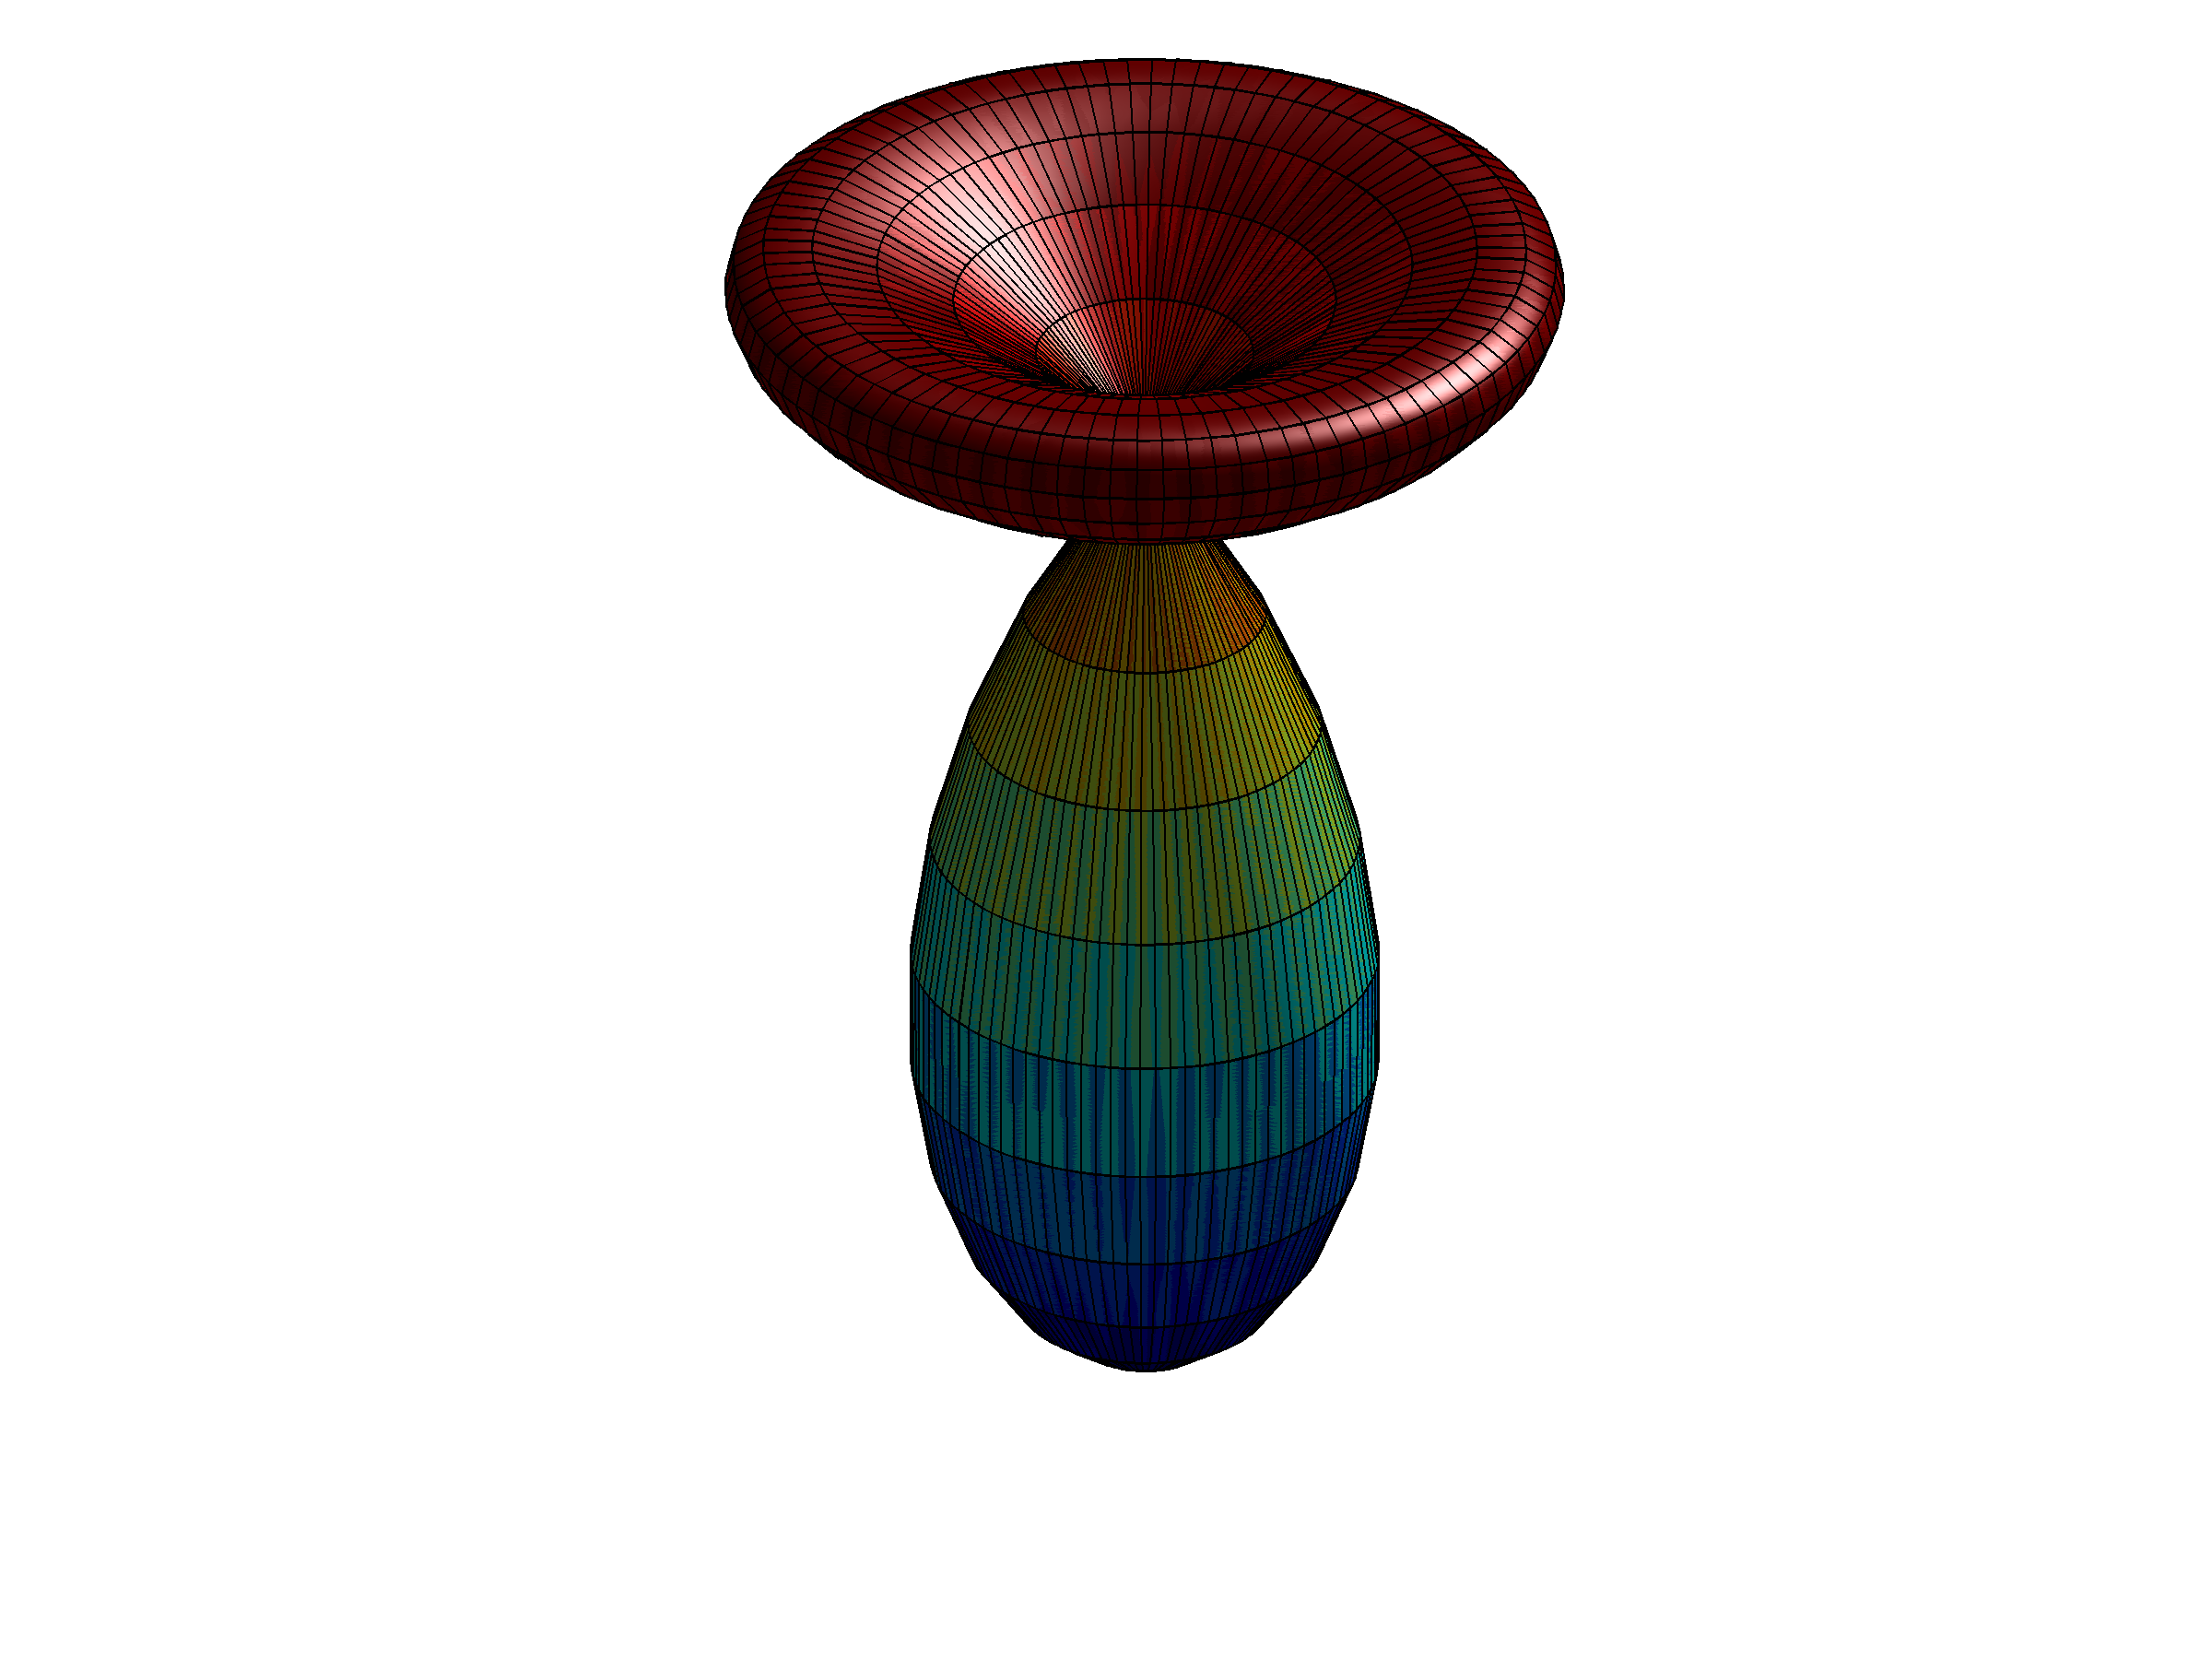
\includegraphics[width=\textwidth]{figures/appendices/Y_3_0.png}
		\caption{}
	\end{subfigure}
	\vfill
	\begin{subfigure}[b]{0.40\textwidth}
		\centering
		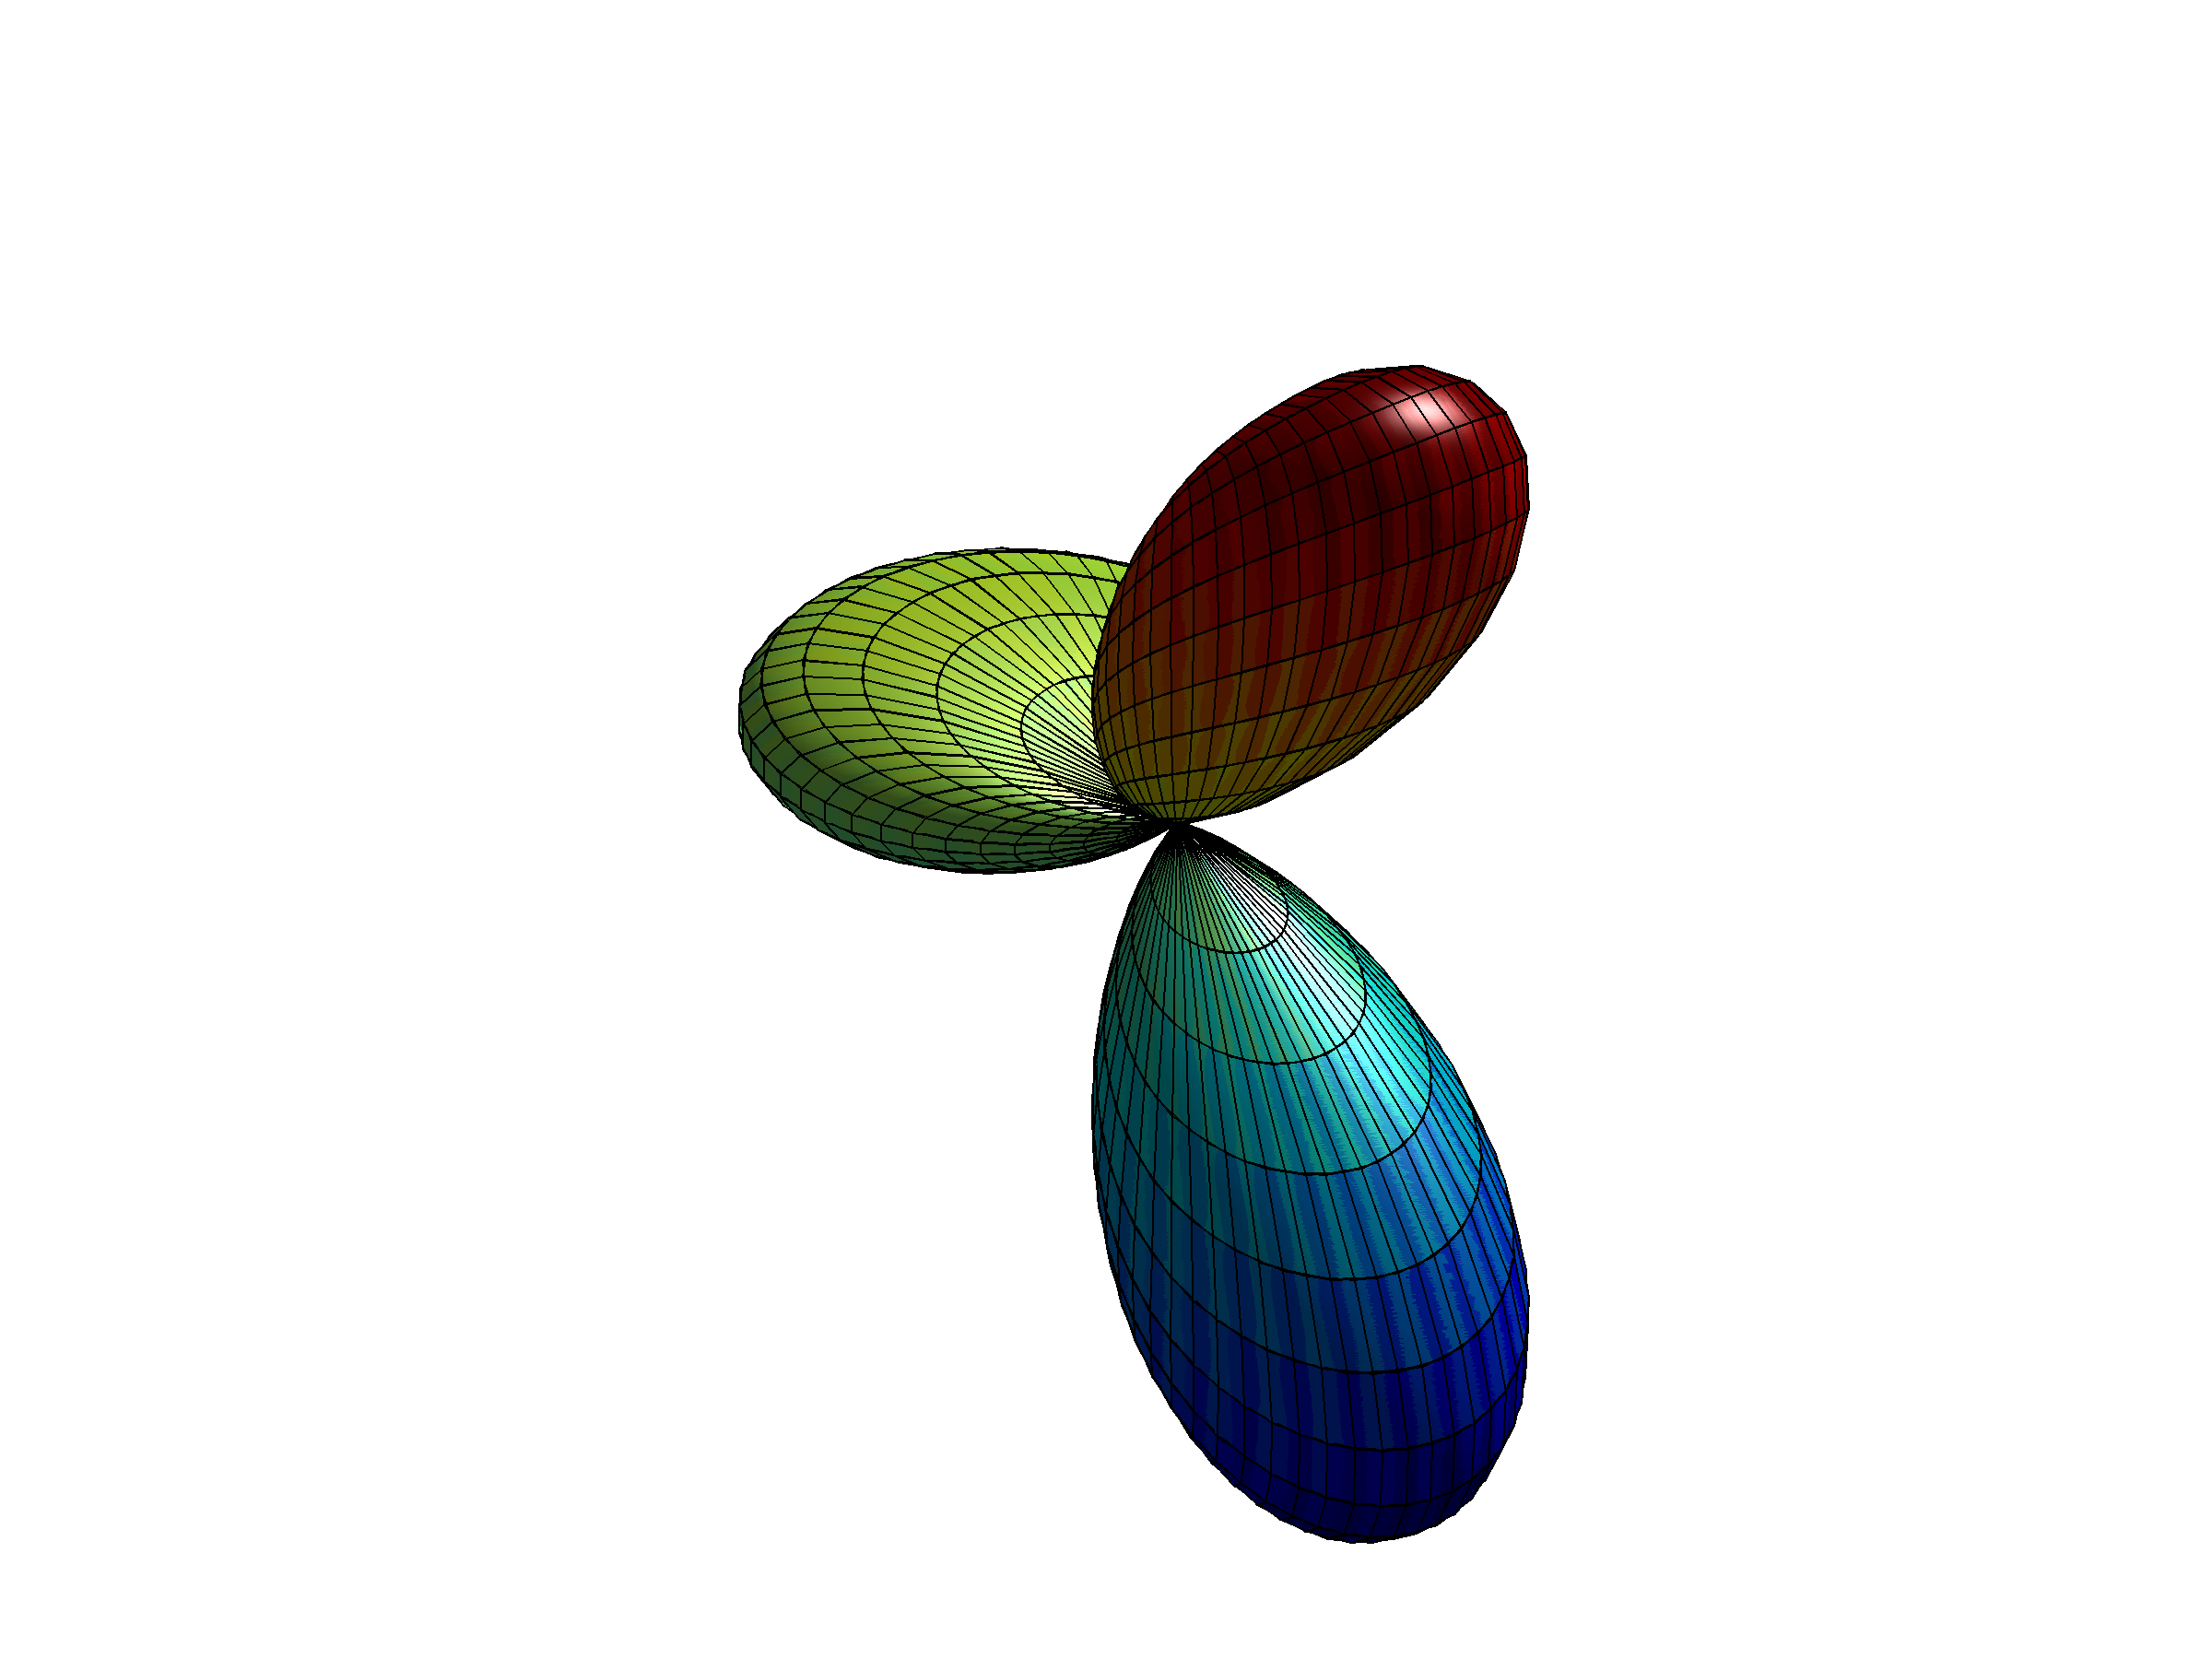
\includegraphics[width=\textwidth]{figures/appendices/Y_3_-1.png}
		\caption{}
	\end{subfigure}
	\hfill
	\begin{subfigure}[b]{0.40\textwidth}
		\centering
		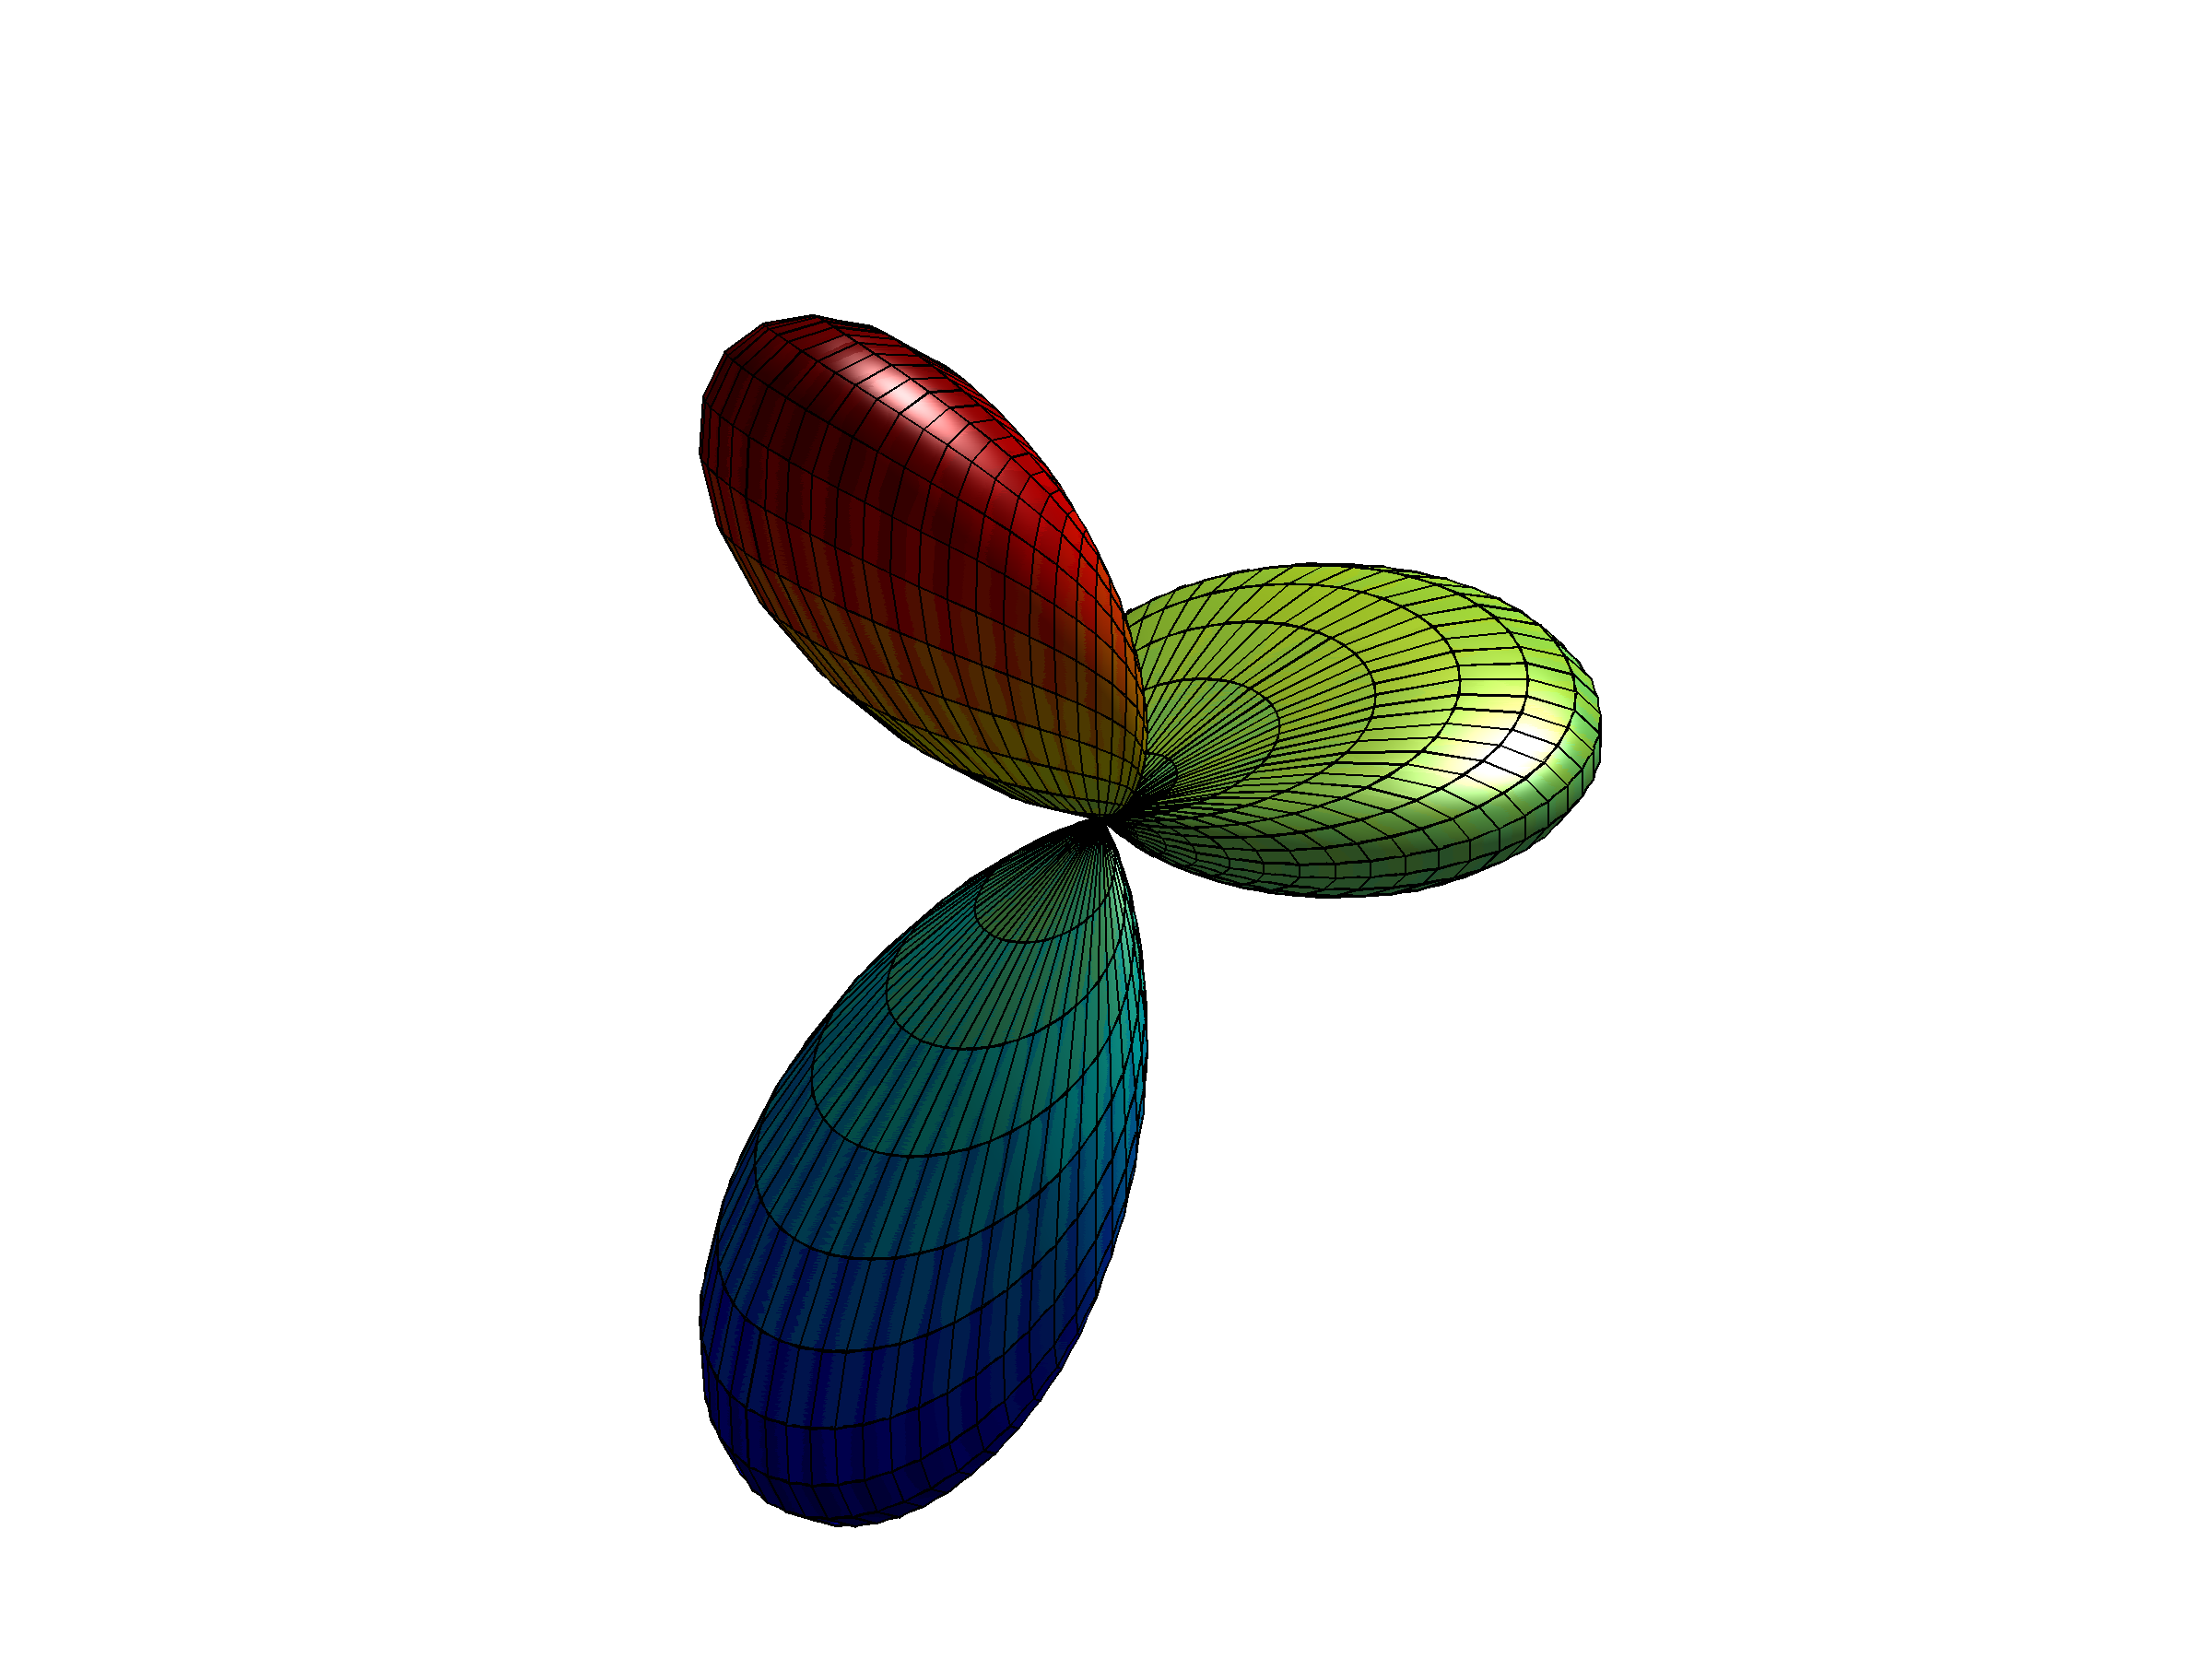
\includegraphics[width=\textwidth]{figures/appendices/Y_3_1.png}
		\caption{}
	\end{subfigure}
	\vfill
	\begin{subfigure}[b]{0.40\textwidth}
		\centering
		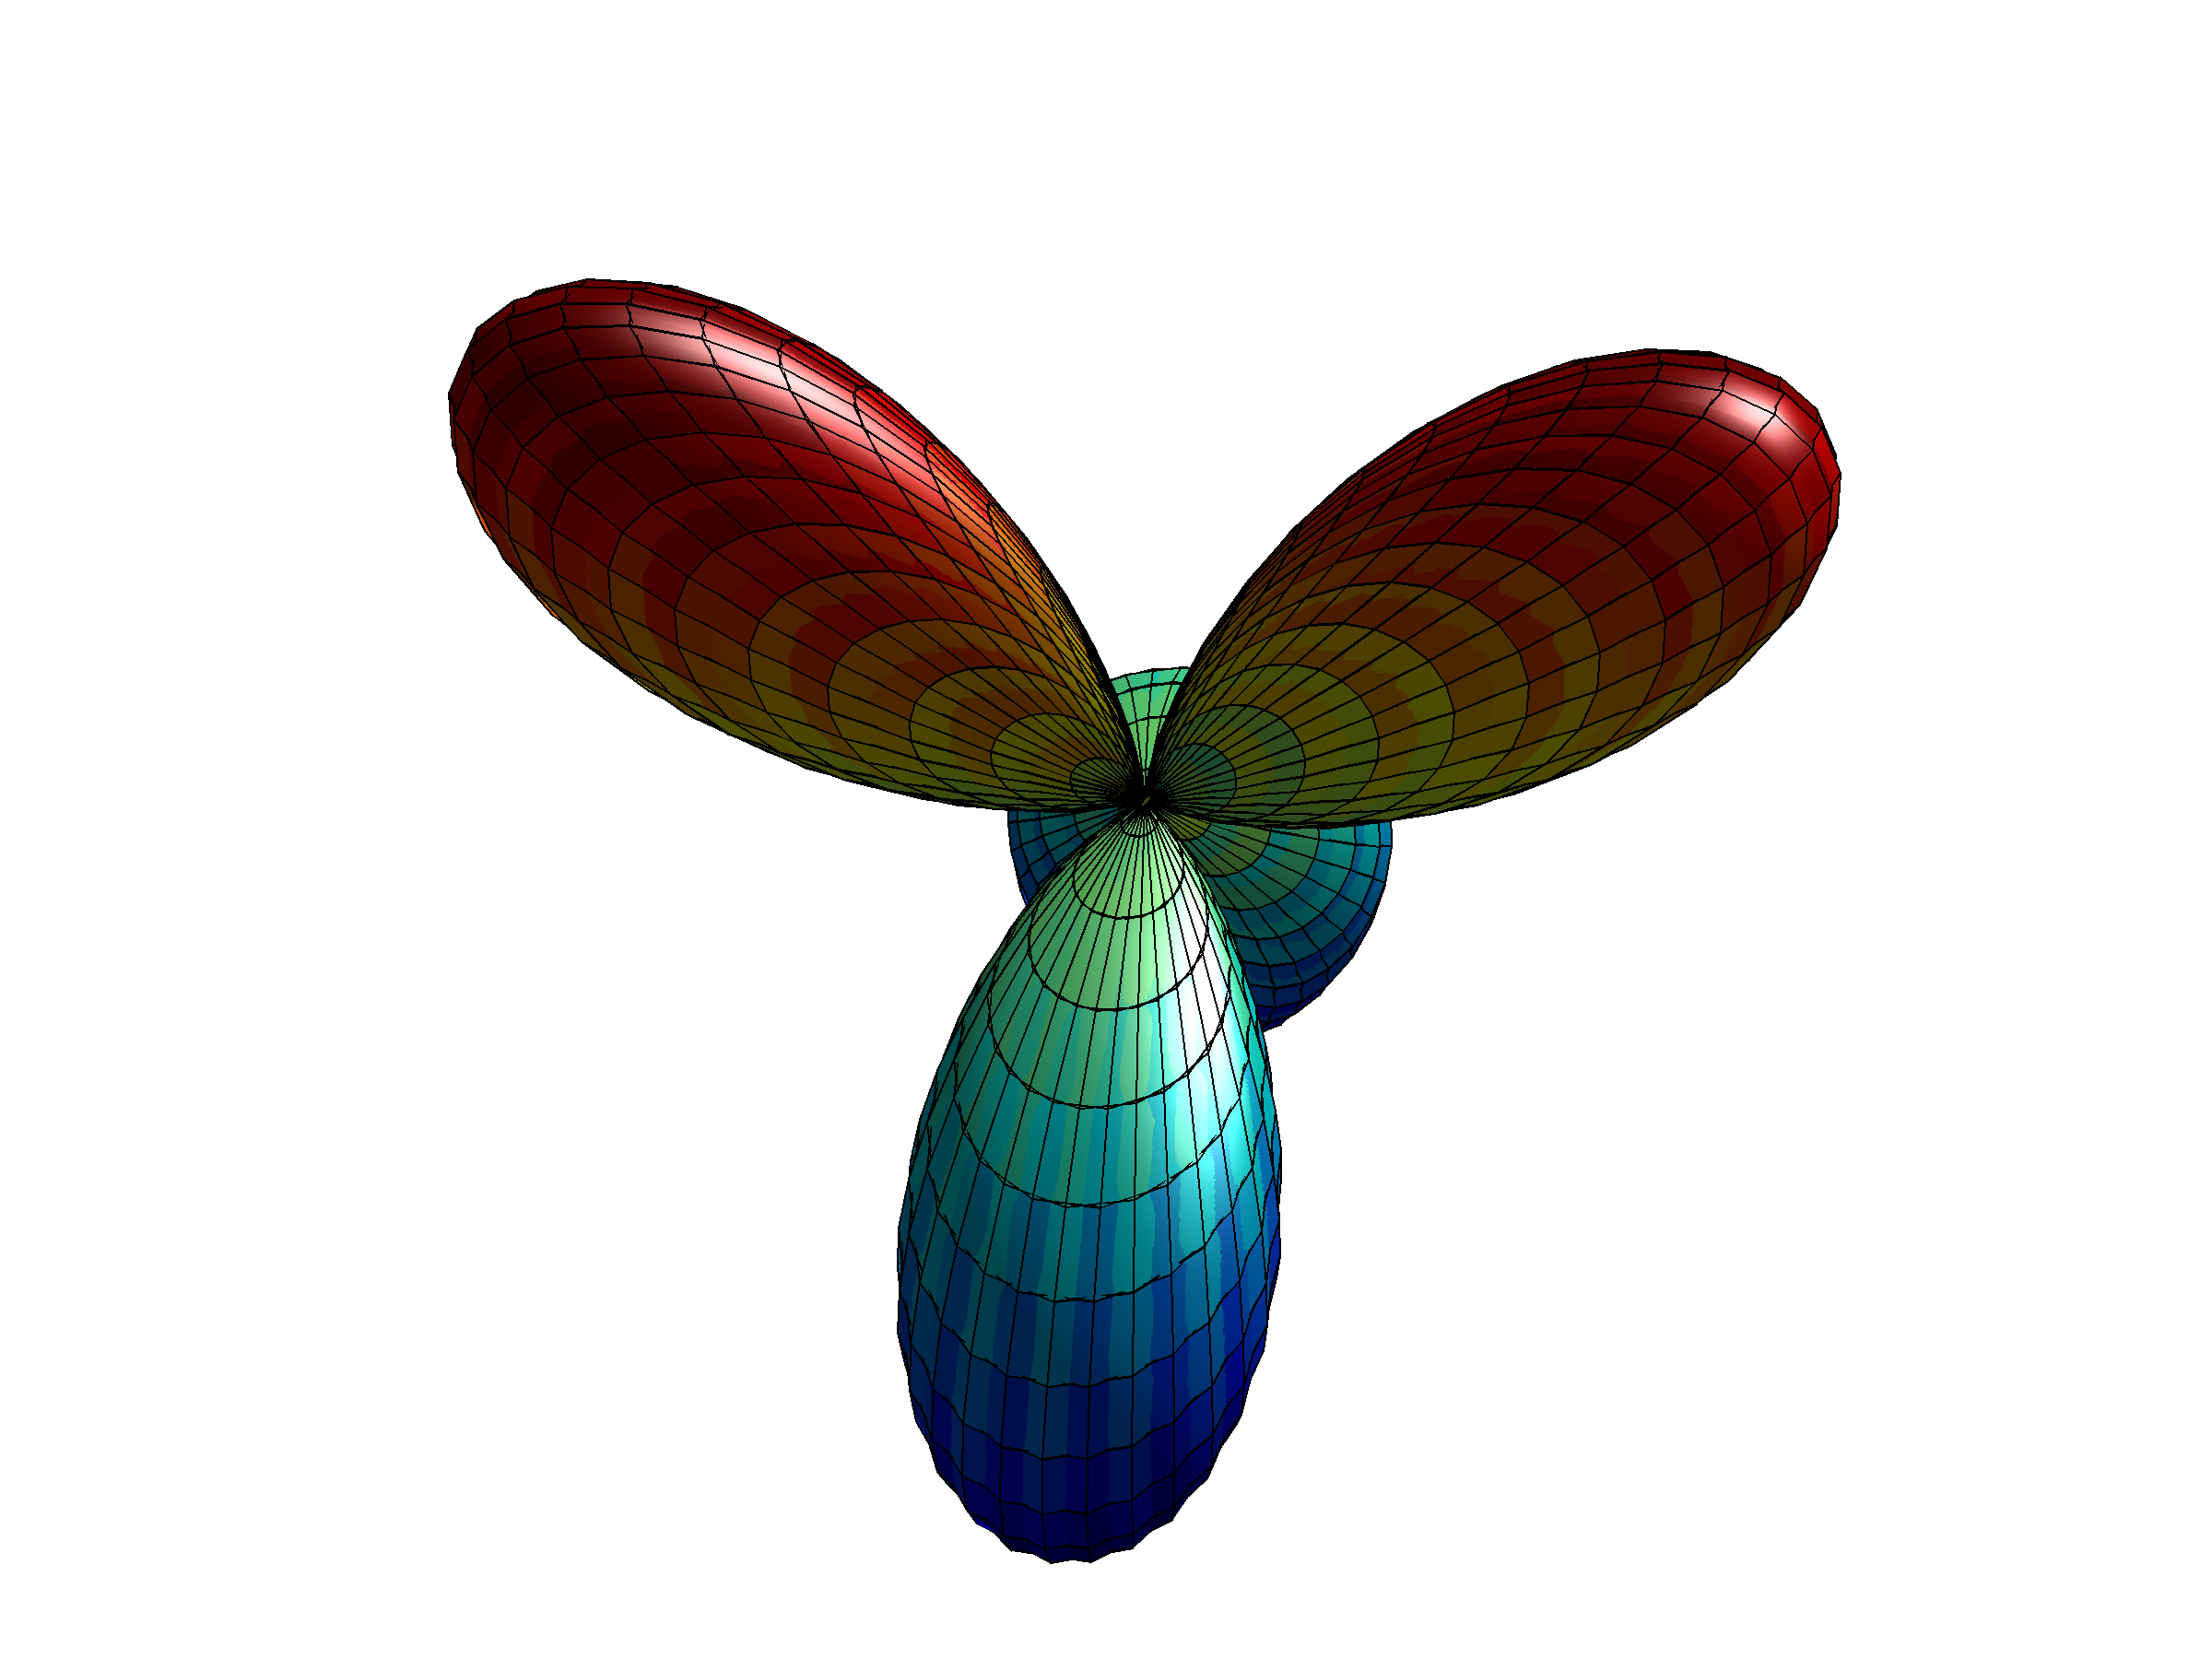
\includegraphics[width=\textwidth]{figures/appendices/Y_3_-2.png}
		\caption{}
	\end{subfigure}
	\hfill
	\begin{subfigure}[b]{0.40\textwidth}
		\centering
		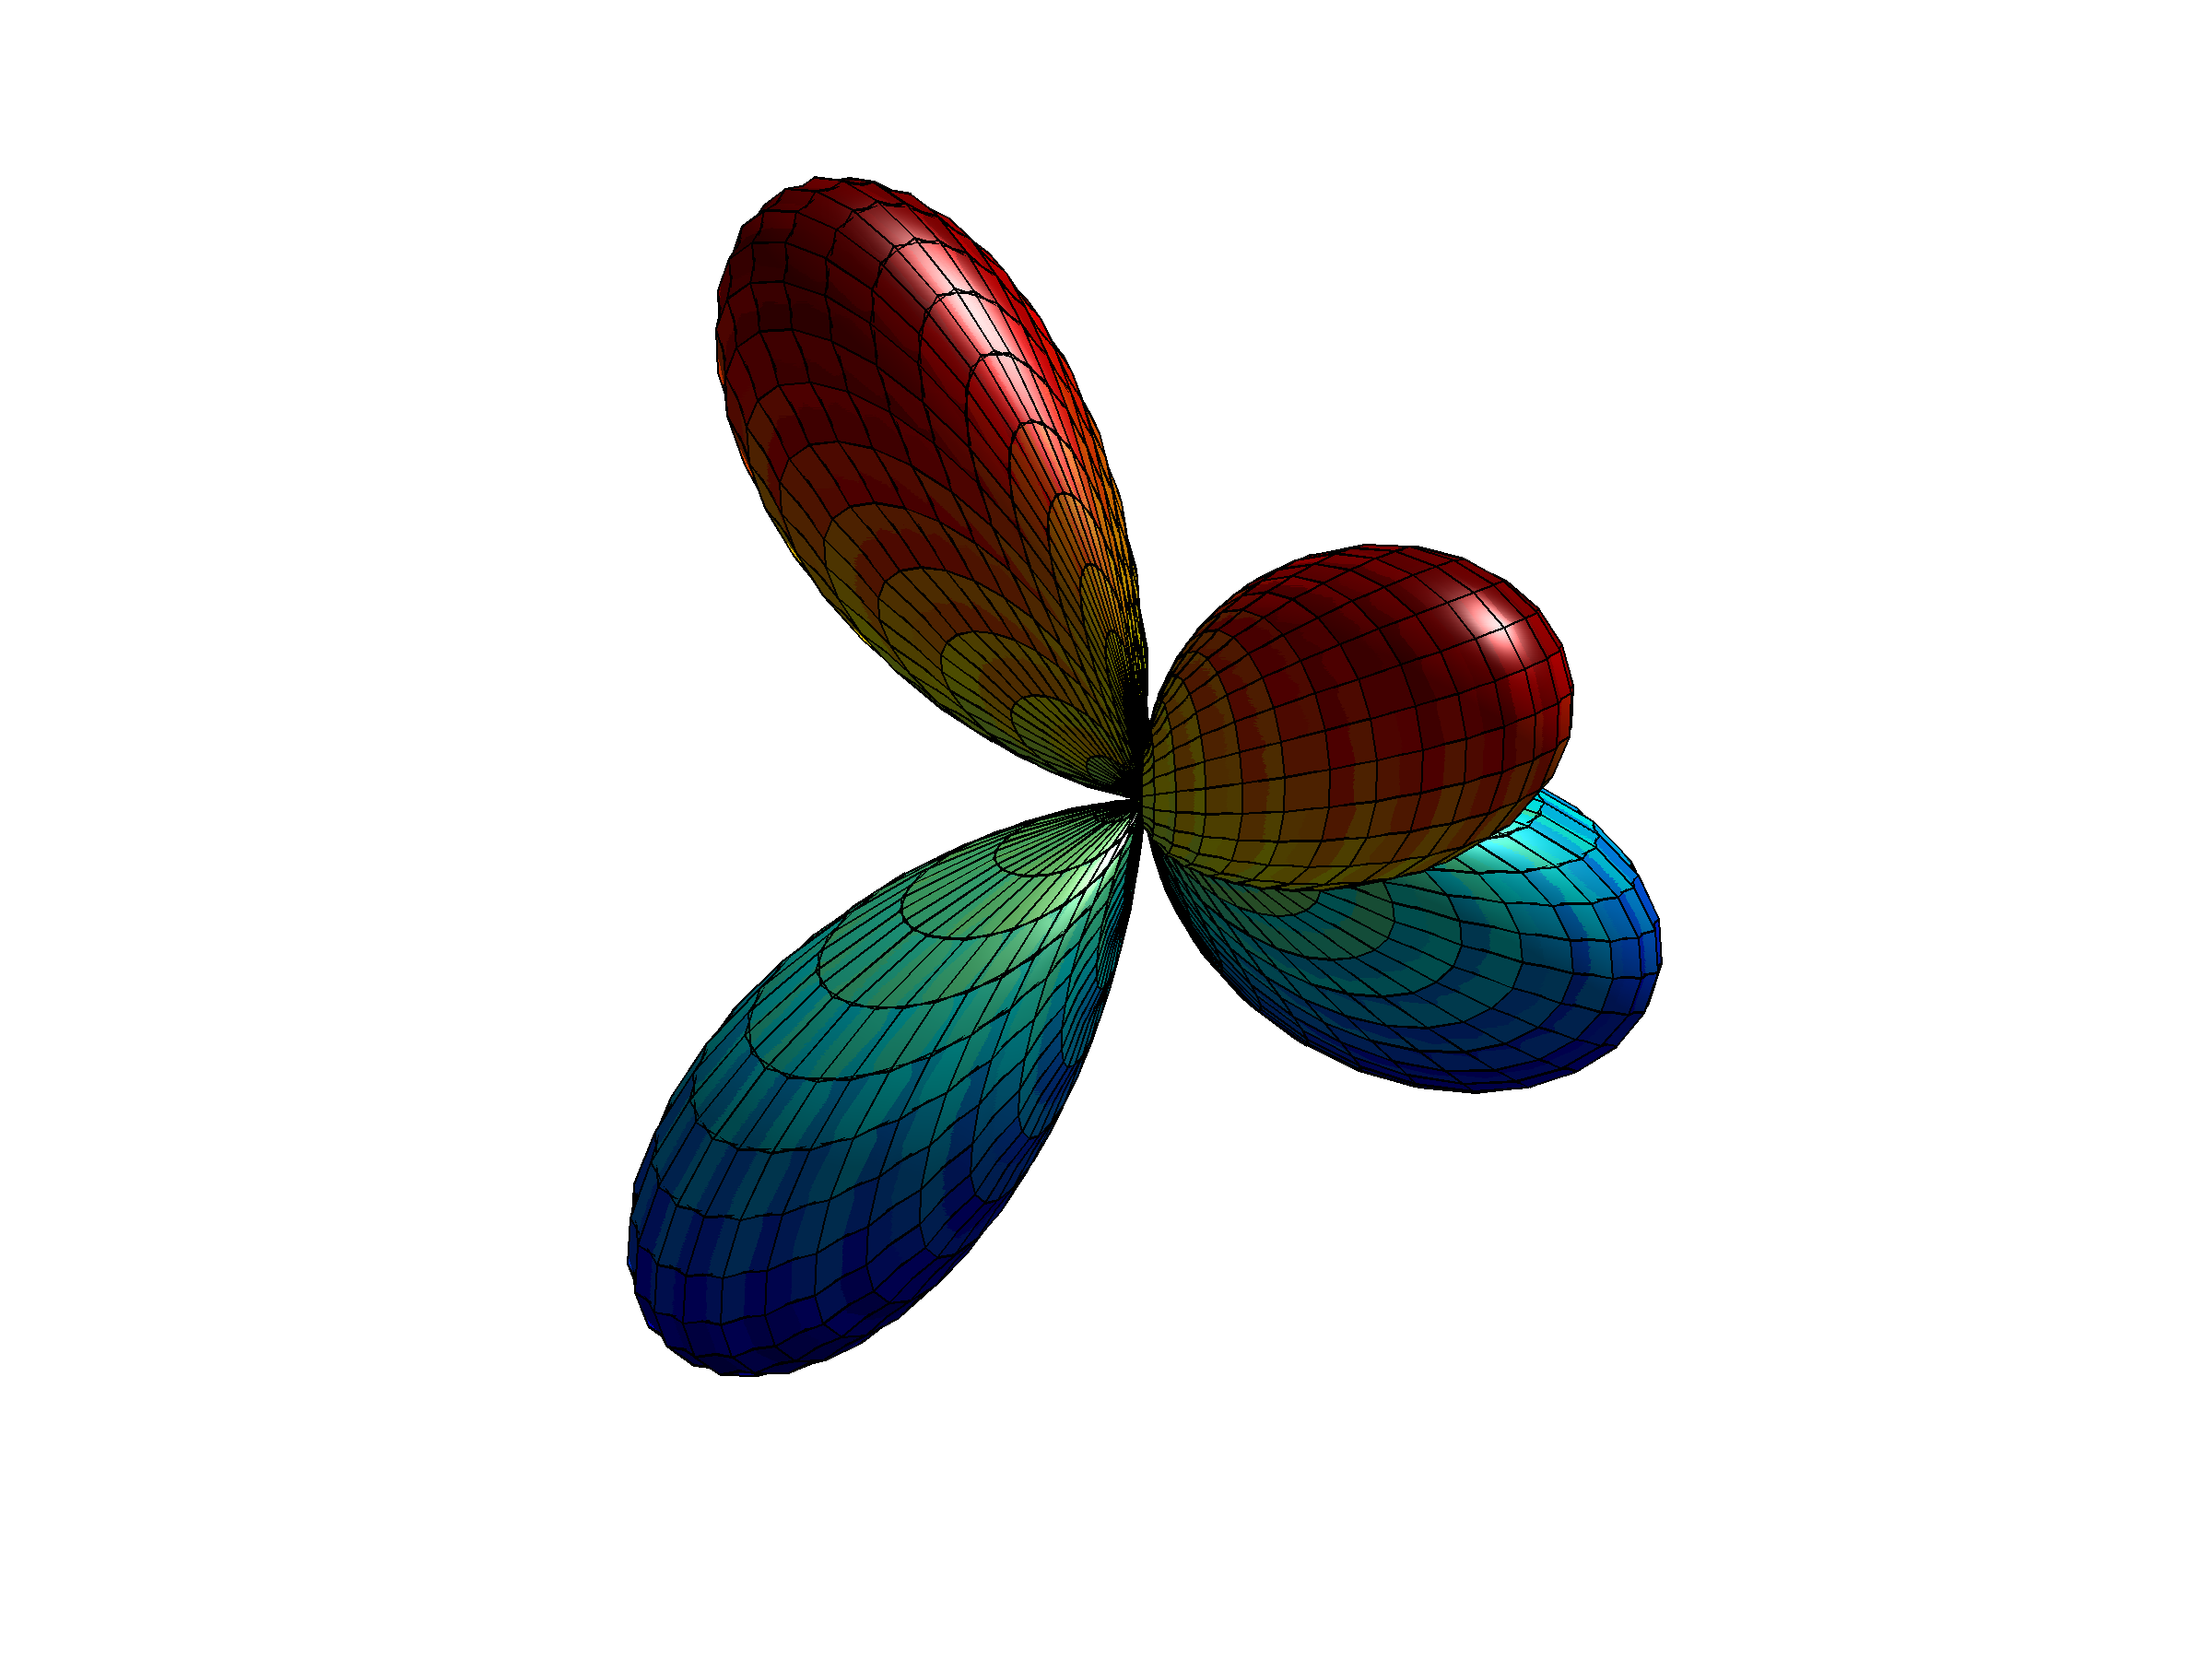
\includegraphics[width=\textwidth]{figures/appendices/Y_3_2.png}
		\caption{}
	\end{subfigure}
	\vfill
	\begin{subfigure}[b]{0.40\textwidth}
		\centering
		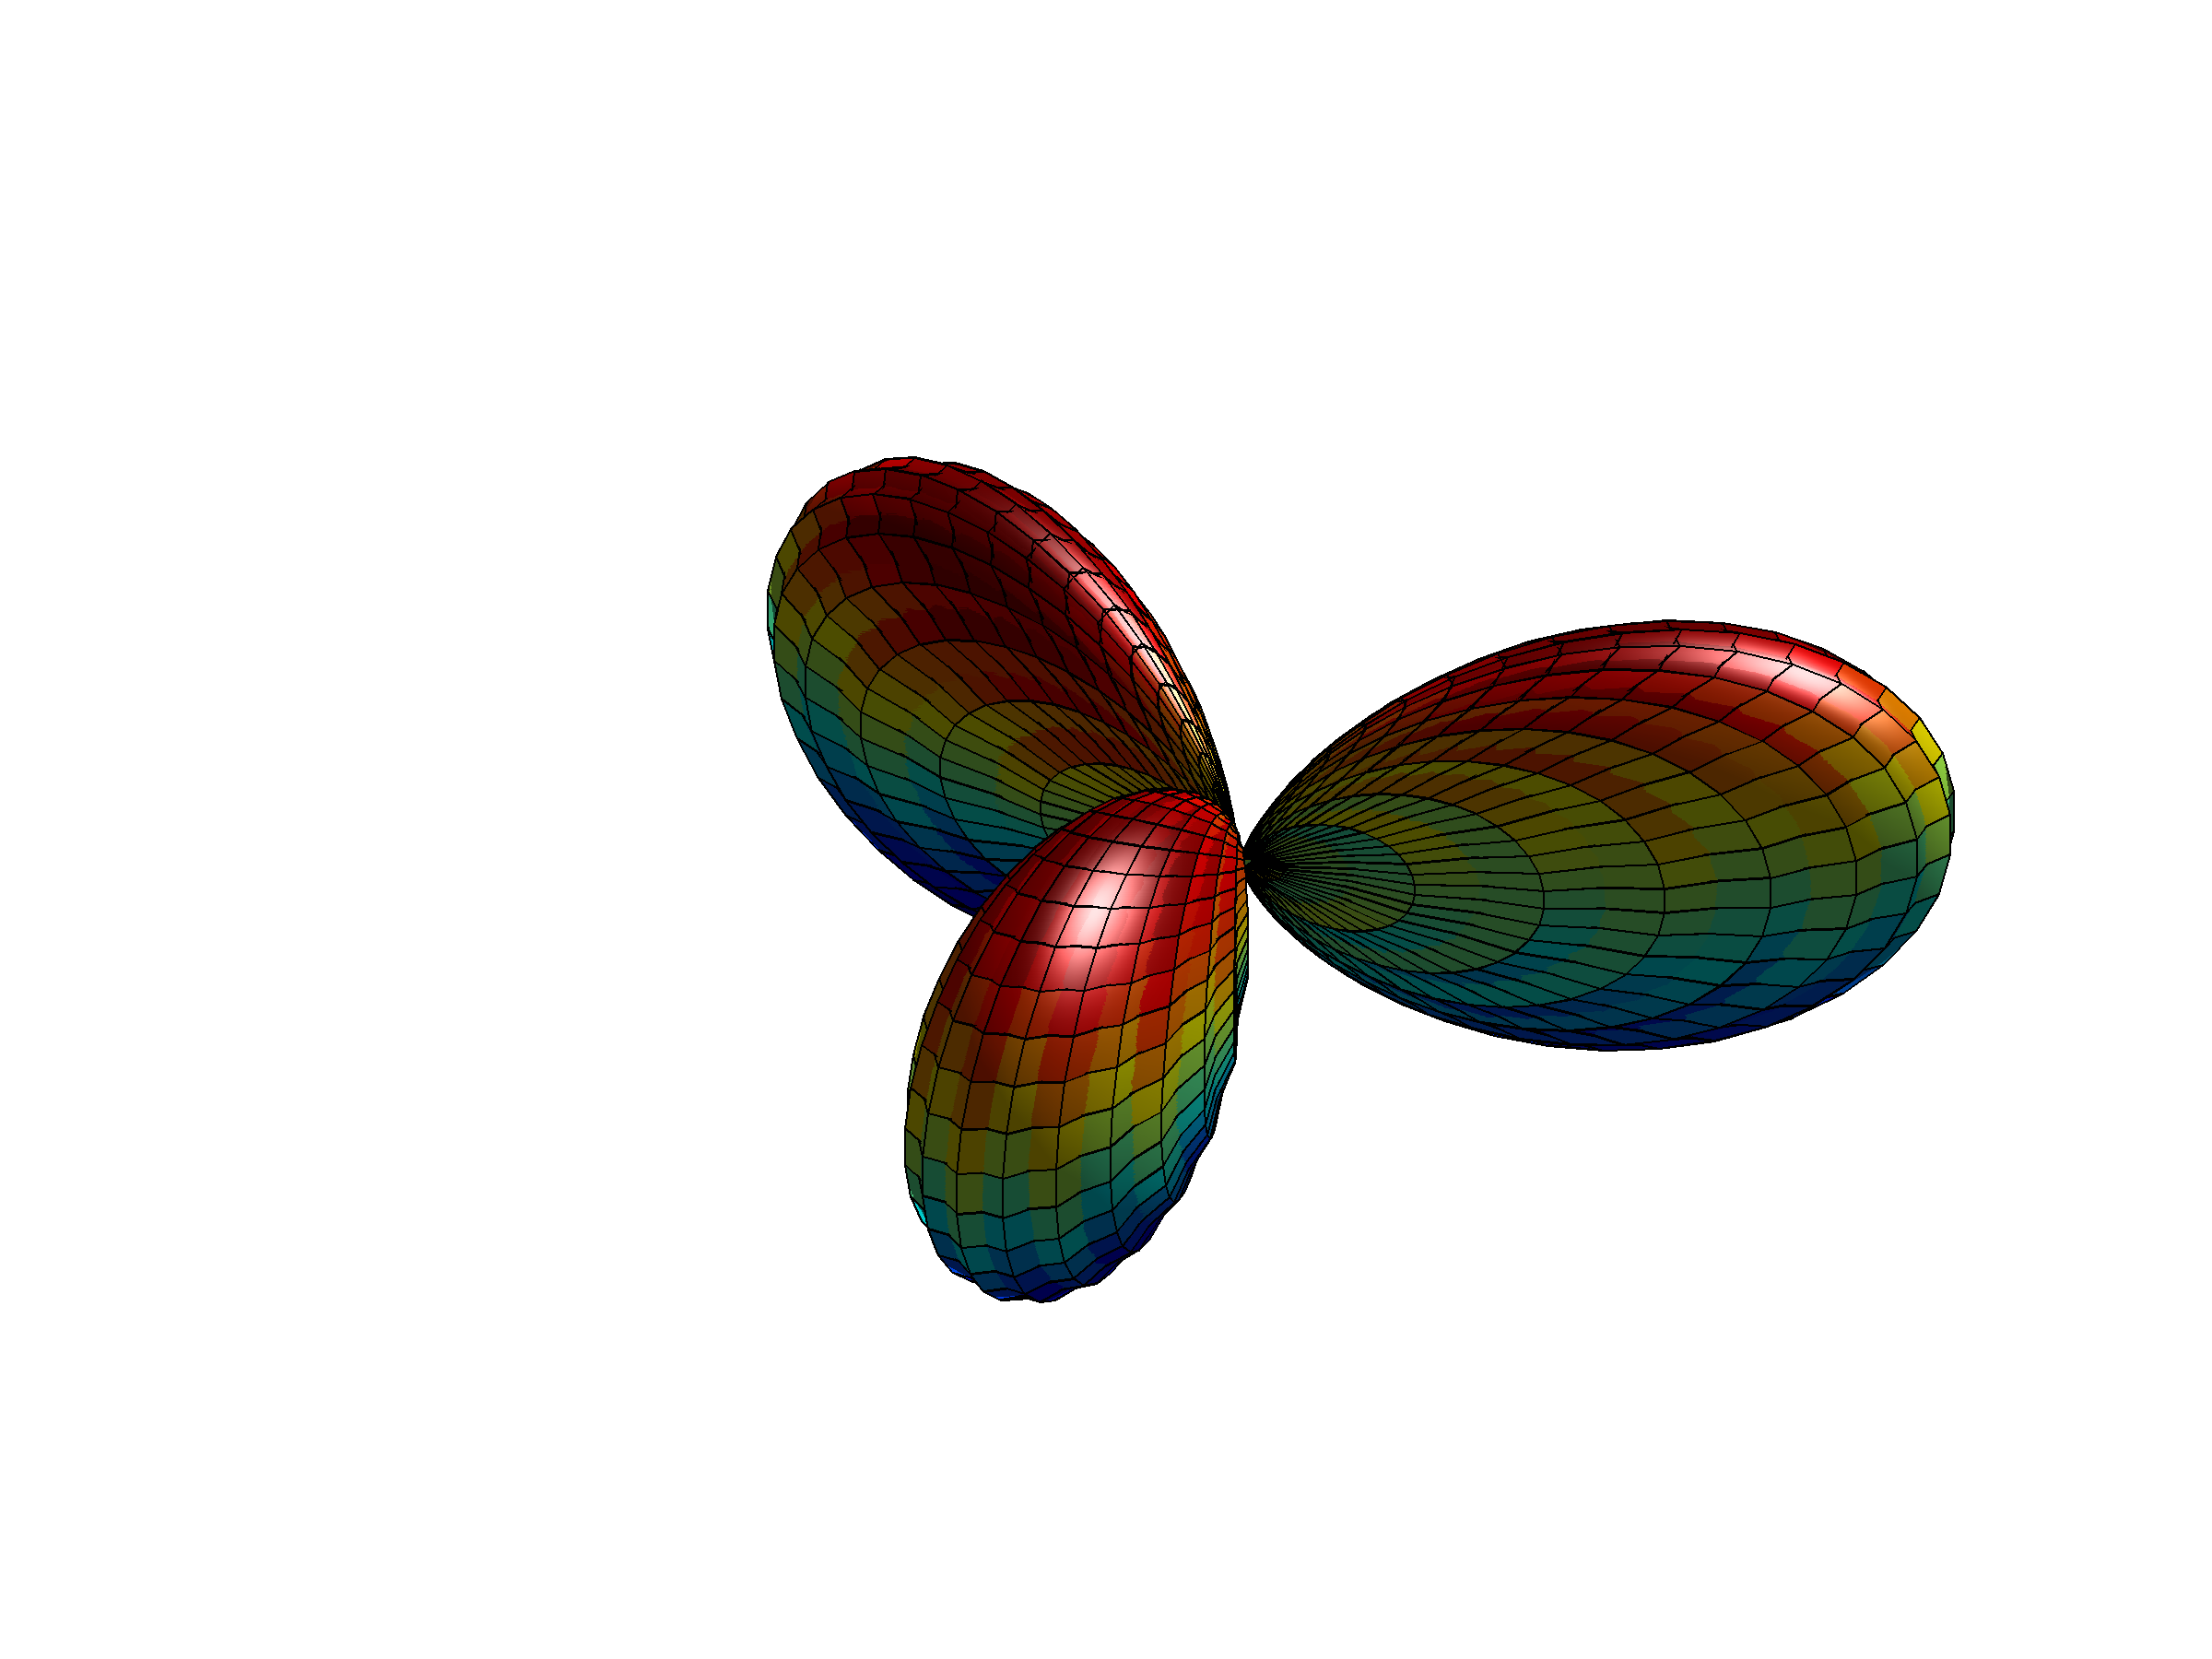
\includegraphics[width=\textwidth]{figures/appendices/Y_3_-3.png}
		\caption{}
	\end{subfigure}
	\hfill
	\begin{subfigure}[b]{0.40\textwidth}
		\centering
		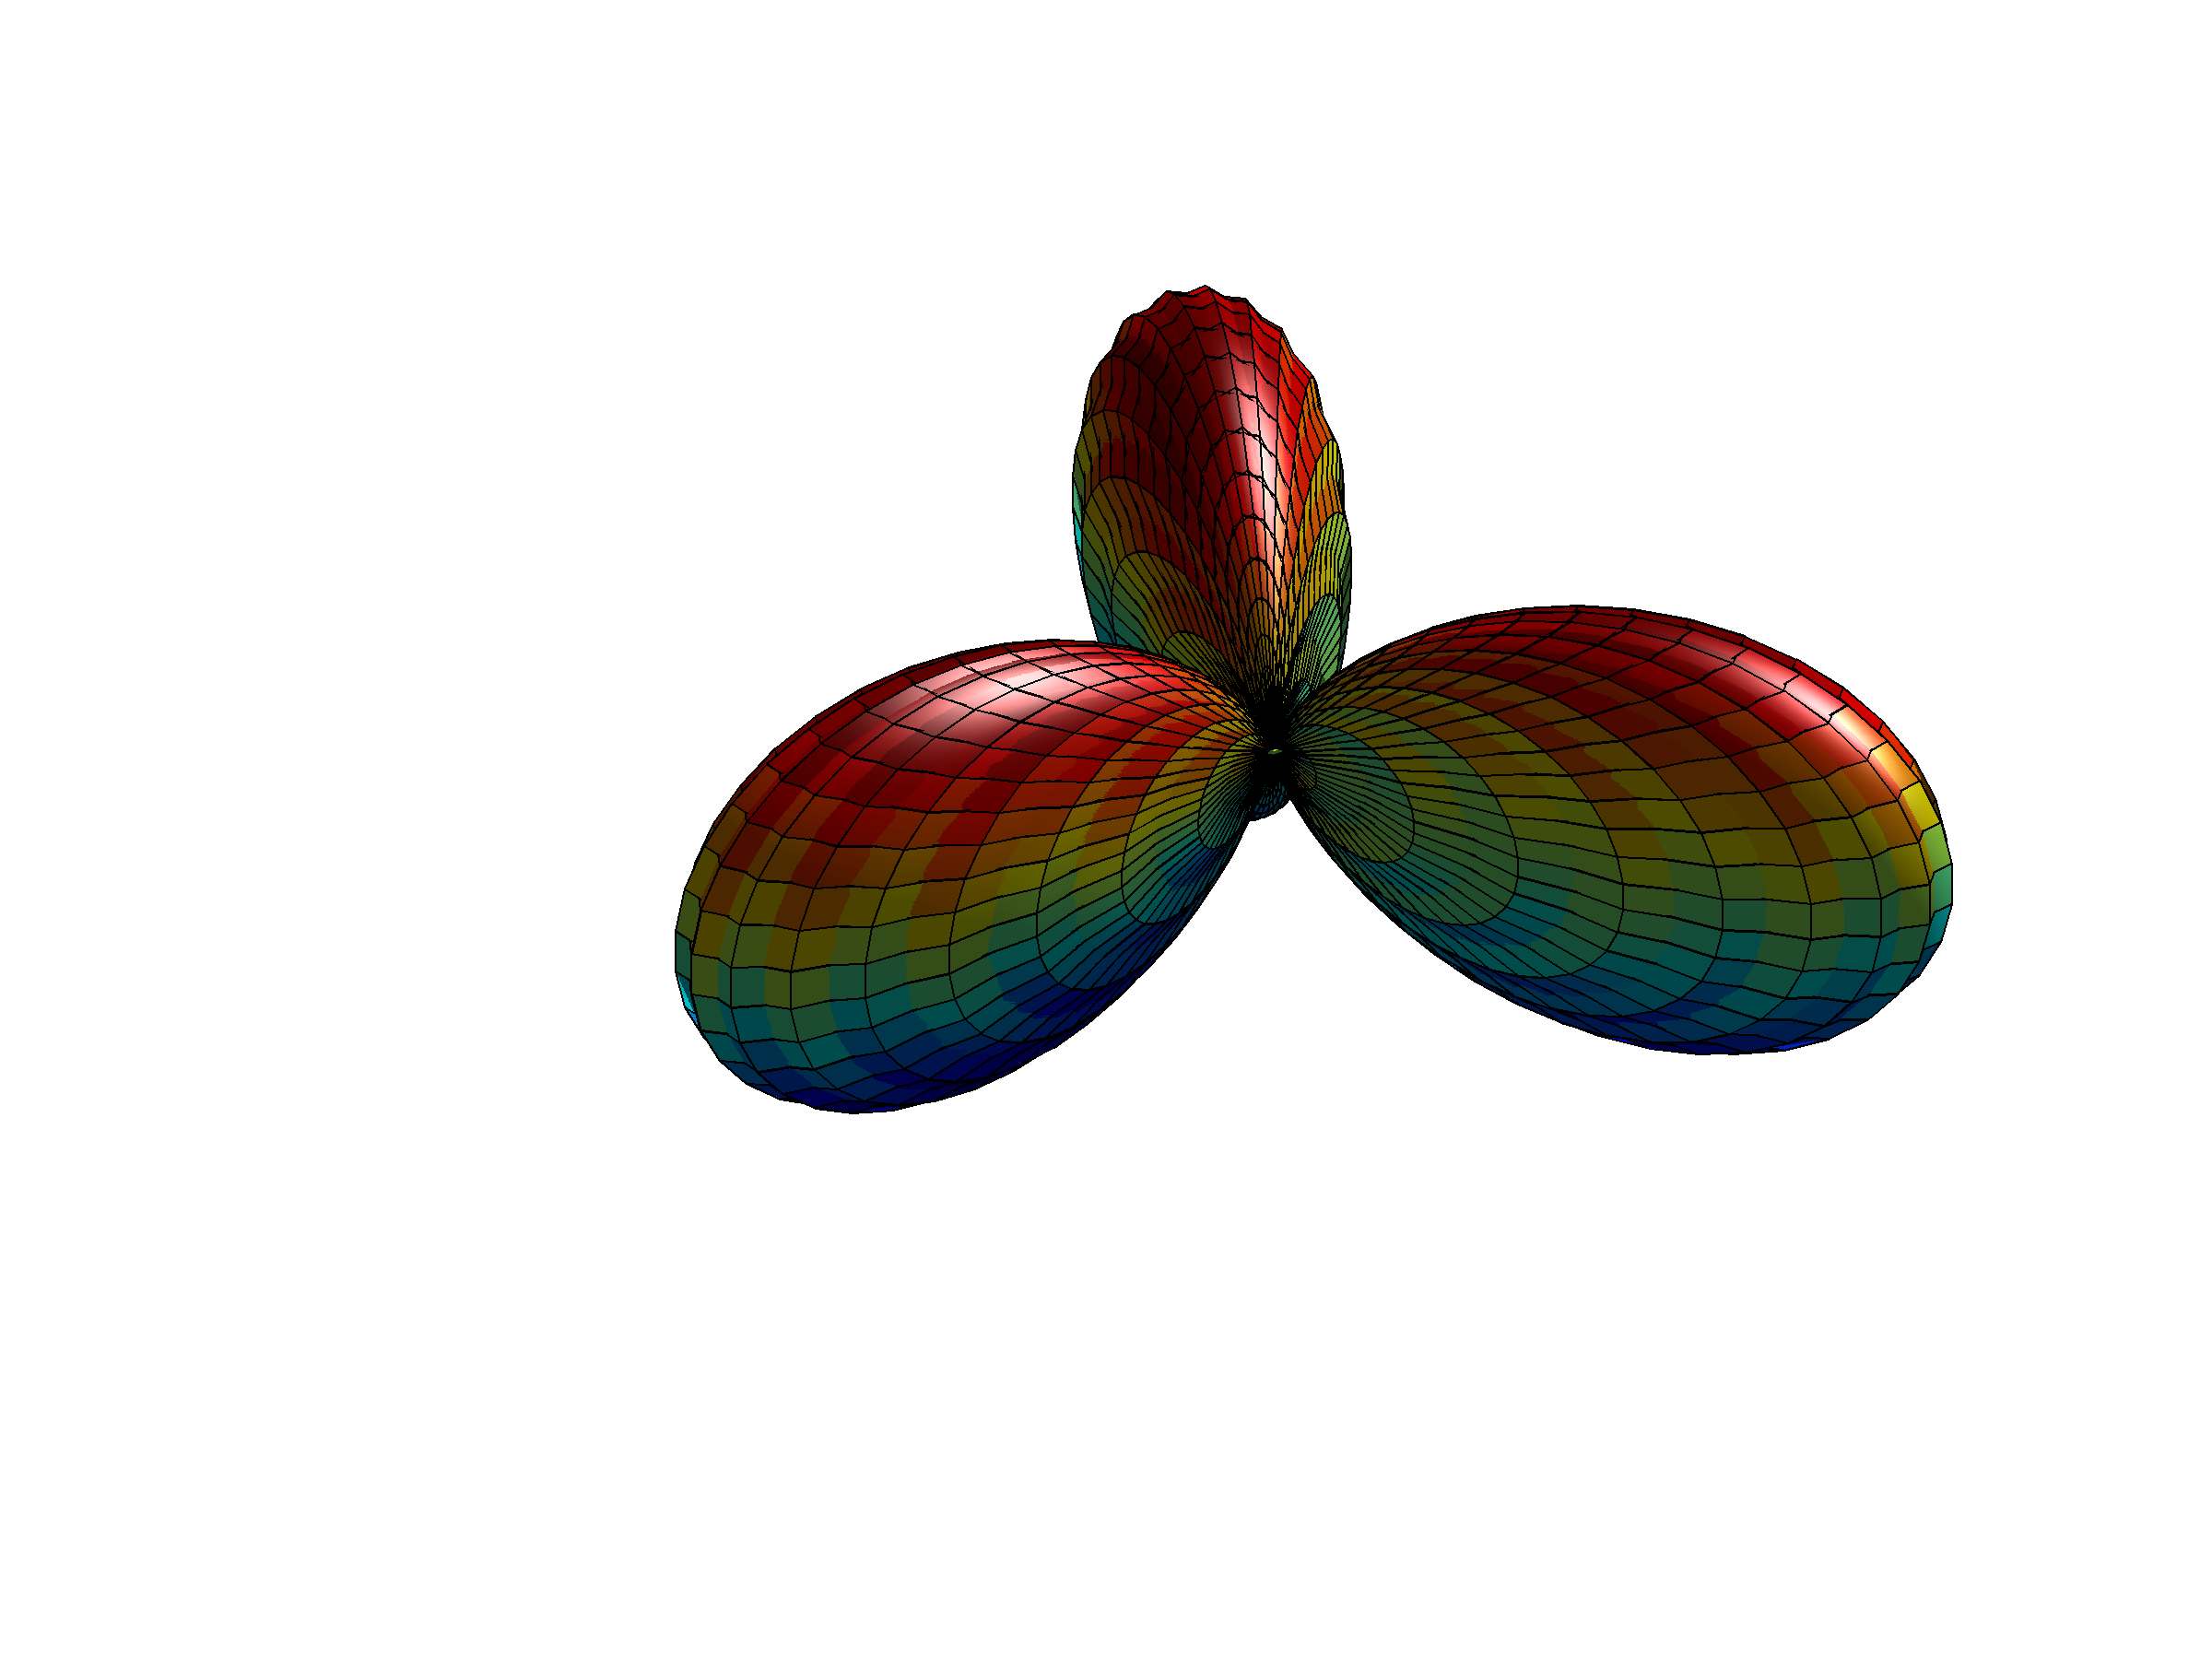
\includegraphics[width=\textwidth]{figures/appendices/Y_3_3.png}
		\caption{}
	\end{subfigure}
\caption{Spherical harmonic functions of degree 3: (a) $Y_{3}^{0}$, (b) $Y_{3}^{-1}$, (c) $Y_{3}^{1}$, (d) $Y_{3}^{-2}$, (e) $Y_{3}^{2}$, (f) $Y_{3}^{-3}$, and (g) $Y_{3}^{3}$.}
\end{figure}

\fi